% **************************************************************************************************************
% A Classic Thesis Style
% An Homage to The Elements of Typographic Style
%
% Copyright (C) 2015 André Miede http://www.miede.de
%
% If you like the style then I would appreciate a postcard. My address 
% can be found in the file ClassicThesis.pdf. A collection of the 
% postcards I received so far is available online at 
% http://postcards.miede.de
%
% License:
% This program is free software; you can redistribute it and/or modify
% it under the terms of the GNU General Public License as published by
% the Free Software Foundation; either version 2 of the License, or
% (at your option) any later version.
%
% This program is distributed in the hope that it will be useful,
% but WITHOUT ANY WARRANTY; without even the implied warranty of
% MERCHANTABILITY or FITNESS FOR A PARTICULAR PURPOSE.  See the
% GNU General Public License for more details.
%
% You should have received a copy of the GNU General Public License
% along with this program; see the file COPYING.  If not, write to
% the Free Software Foundation, Inc., 59 Temple Place - Suite 330,
% Boston, MA 02111-1307, USA.
%
% **************************************************************************************************************
\RequirePackage{fix-cm} % fix some latex issues see: http://texdoc.net/texmf-dist/doc/latex/base/fixltx2e.pdf
\documentclass[twoside,openright,titlepage,numbers=noenddot,headinclude,%1headlines,% letterpaper a4paper
                footinclude=true,cleardoublepage=empty,abstractoff, % <--- obsolete, remove (todo)
                BCOR=5mm,paper=a4,fontsize=11pt,%11pt,a4paper,%
                ngerman,american,%
                ]{scrreprt}
%\overfullrule=2cm
%********************************************************************
% Note: Make all your adjustments in here
%*******************************************************
% ****************************************************************************************************
% classicthesis-config.tex 
% formerly known as loadpackages.sty, classicthesis-ldpkg.sty, and classicthesis-preamble.sty 
% Use it at the beginning of your ClassicThesis.tex, or as a LaTeX Preamble 
% in your ClassicThesis.{tex,lyx} with % ****************************************************************************************************
% classicthesis-config.tex 
% formerly known as loadpackages.sty, classicthesis-ldpkg.sty, and classicthesis-preamble.sty 
% Use it at the beginning of your ClassicThesis.tex, or as a LaTeX Preamble 
% in your ClassicThesis.{tex,lyx} with % ****************************************************************************************************
% classicthesis-config.tex 
% formerly known as loadpackages.sty, classicthesis-ldpkg.sty, and classicthesis-preamble.sty 
% Use it at the beginning of your ClassicThesis.tex, or as a LaTeX Preamble 
% in your ClassicThesis.{tex,lyx} with \input{classicthesis-config}
% ****************************************************************************************************  
% If you like the classicthesis, then I would appreciate a postcard. 
% My address can be found in the file ClassicThesis.pdf. A collection 
% of the postcards I received so far is available online at 
% http://postcards.miede.de
% ****************************************************************************************************


% ****************************************************************************************************
% 0. Set the encoding of your files. UTF-8 is the only sensible encoding nowadays. If you can't read
% äöüßáéçèê∂åëæƒÏ€ then change the encoding setting in your editor, not the line below. If your editor
% does not support utf8 use another editor!
% ****************************************************************************************************
\PassOptionsToPackage{utf8}{inputenc}
	\usepackage{inputenc}

% ****************************************************************************************************
% 1. Configure classicthesis for your needs here, e.g., remove "drafting" below 
% in order to deactivate the time-stamp on the pages
% ****************************************************************************************************
\PassOptionsToPackage{eulerchapternumbers,drafting,%listings
                      pdfspacing,%floatperchapter,%linedheaders,%
		      subfig,beramono,eulermath,parts,}
                     {classicthesis}                                        
% ********************************************************************
% Available options for classicthesis.sty 
% (see ClassicThesis.pdf for more information):
% drafting
% parts nochapters linedheaders
% eulerchapternumbers beramono eulermath pdfspacing minionprospacing
% tocaligned dottedtoc manychapters
% listings floatperchapter subfig
% ********************************************************************


% ****************************************************************************************************
% 2. Personal data and user ad-hoc commands
% ****************************************************************************************************
\newcommand{\myTitle}{Diseño e implementación de un analizador de dependencias para procesamiento de lenguaje natural en Español\xspace}
\newcommand{\mySubtitle}{Mediante Máquinas de Soporte Vectoriales\xspace}
\newcommand{\myDegree}{Grado en Ingeniería Informática\xspace}
\newcommand{\myName}{Alejandro Alcalde Barros\xspace}
\newcommand{\myProf}{Salvador García López\xspace}
\newcommand{\myOtherProf}{Put name here\xspace}
\newcommand{\mySupervisor}{Put name here\xspace}
\newcommand{\myFaculty}{Escuela Técnica Superior de Ingenierías Informática y de Telecomunicación\xspace}
\newcommand{\myDepartment}{DECSAI\xspace}
\newcommand{\myUni}{Universidad de Granada\xspace}
\newcommand{\myLocation}{Granada\xspace}
\newcommand{\myTime}{\today\xspace}
\newcommand{\myVersion}{version 4.2\xspace}

% ********************************************************************
% Setup, finetuning, and useful commands
% ********************************************************************
\newcounter{dummy} % necessary for correct hyperlinks (to index, bib, etc.)
\newlength{\abcd} % for ab..z string length calculation
\providecommand{\mLyX}{L\kern-.1667em\lower.25em\hbox{Y}\kern-.125emX\@}
\newcommand{\ie}{i.\,e.}
\newcommand{\Ie}{I.\,e.}
\newcommand{\eg}{por ejemplo,}
\newcommand{\Eg}{E.\,g.} 
% ****************************************************************************************************


% ****************************************************************************************************
% 3. Loading some handy packages
% ****************************************************************************************************
% ******************************************************************** 
% Packages with options that might require adjustments
% ******************************************************************** 
\PassOptionsToPackage{spanish,american}{babel}   % change this to your language(s)
% Spanish languages need extra options in order to work with this template
\PassOptionsToPackage{spanish,es-lcroman}{babel}
\usepackage[spanish,es-tabla]{babel}

\usepackage{csquotes}
\PassOptionsToPackage{%
    %backend=biber, %instead of bibtex
	backend=bibtex8,bibencoding=ascii,%
	language=auto,%
	style=numeric-comp,%
    %style=authoryear-comp, % Author 1999, 2010
    %bibstyle=authoryear,dashed=false, % dashed: substitute rep. author with ---
    sorting=nyt, % name, year, title
    maxbibnames=10, % default: 3, et al.
    %backref=true,%
    natbib=true % natbib compatibility mode (\citep and \citet still work)
}{biblatex}
    \usepackage{biblatex}

\PassOptionsToPackage{fleqn}{amsmath}       % math environments and more by the AMS 
    \usepackage{amsmath}

% ******************************************************************** 
% General useful packages
% ******************************************************************** 
\PassOptionsToPackage{T1}{fontenc} % T2A for cyrillics
    \usepackage{fontenc}     
\usepackage{textcomp} % fix warning with missing font shapes
\usepackage{scrhack} % fix warnings when using KOMA with listings package          
\usepackage{xspace} % to get the spacing after macros right  
\usepackage{mparhack} % get marginpar right
\usepackage{fixltx2e} % fixes some LaTeX stuff --> since 2015 in the LaTeX kernel (see below)
%\usepackage[latest]{latexrelease} % will be used once available in more distributions (ISSUE #107)
\PassOptionsToPackage{printonlyused,smaller}{acronym} 
    \usepackage{acronym} % nice macros for handling all acronyms in the thesis
    %\renewcommand{\bflabel}[1]{{#1}\hfill} % fix the list of acronyms --> no longer working
    %\renewcommand*{\acsfont}[1]{\textsc{#1}} 
    \renewcommand*{\aclabelfont}[1]{\acsfont{#1}}

%%%%%%%%%%%%%%%%%%%%%%%%%%%%%%%%%%%%%%%%%%%%%%%%%%%%%%
%%%%%%%%%%%%%%% Added by myself %%%%%%%%%%%%%%%%%%%%%%
%%%%%%%%%%%%%%%%%%%%%%%%%%%%%%%%%%%%%%%%%%%%%%%%%%%%%%
\usepackage{xargs}                      % Use more than one optional parameter in a new commands
\usepackage[pdftex,dvipsnames,table,xcdraw]{xcolor}  % Coloured text etc.
\definecolor{bugColor}{HTML}{fc221b}
\definecolor{enhancementColor}{HTML}{84979b}
\definecolor{questionColor}{HTML}{cc2952}
\definecolor{todoColor}{HTML}{fba803}

\usepackage[colorinlistoftodos,prependcaption,textsize=scriptsize,english]{todonotes}
\newcommandx{\bug}[2][1=]{\todo[linecolor=bugColor,backgroundcolor=bugColor!25,bordercolor=bugColor,#1]{#2}}
\newcommandx{\enhancement}[2][1=]{\todo[linecolor=enhancementColor,backgroundcolor=enhancementColor!25,bordercolor=enhancementColor,#1]{#2}}
\newcommandx{\question}[2][1=]{\todo[linecolor=questionColor,backgroundcolor=questionColor!25,bordercolor=questionColor,#1]{#2}}
\newcommandx{\myTodo}[2][1=]{\todo[linecolor=todoColor,backgroundcolor=todoColor!25,bordercolor=todoColor,#1]{#2}}
\newcommandx{\thiswillnotshow}[2][1=]{\todo[disable,#1]{#2}}

\usepackage{tikz-dependency}
\usepackage{tikz-qtree,tikz-qtree-compat}
\usetikzlibrary{shapes.geometric,arrows,decorations.markings,babel}
\usepackage{tikz-uml}
\usepackage{algorithm}% http://ctan.org/pkg/algorithms
\usepackage{algpseudocode}% http://ctan.org/pkg/algorithmicx
\makeatletter
\renewcommand*{\ALG@name}{Algoritmo}
\makeatother
\usepackage{pgfgantt}
%%%%%%%%%%%%%%%%%%%%%%%%%%%%%%%%%%%%%%%%%%%%%%%%%%%%%%
%%%%%%%%%%%%%%% End Added by myself %%%%%%%%%%%%%%%%%%
%%%%%%%%%%%%%%%%%%%%%%%%%%%%%%%%%%%%%%%%%%%%%%%%%%%%%%
% ****************************************************************************************************


% ****************************************************************************************************
% 4. Setup floats: tables, (sub)figures, and captions
% ****************************************************************************************************
\usepackage{tabularx} % better tables
    \setlength{\extrarowheight}{3pt} % increase table row height
\newcommand{\tableheadline}[1]{\multicolumn{1}{c}{\spacedlowsmallcaps{#1}}}
\newcommand{\myfloatalign}{\centering} % to be used with each float for alignment
\usepackage{caption}
% Thanks to cgnieder and Claus Lahiri
% http://tex.stackexchange.com/questions/69349/spacedlowsmallcaps-in-caption-label
% [REMOVED DUE TO OTHER PROBLEMS, SEE ISSUE #82]    
%\DeclareCaptionLabelFormat{smallcaps}{\bothIfFirst{#1}{~}\MakeTextLowercase{\textsc{#2}}}
%\captionsetup{font=small,labelformat=smallcaps} % format=hang,
\captionsetup{font=small} % format=hang,
\usepackage{subfig}  
% ****************************************************************************************************


% ****************************************************************************************************
% 5. Setup code listings
% ****************************************************************************************************
\usepackage{minted}
\usemintedstyle{tango}
\renewcommand{\listingscaption}{Código}
\renewcommand{\listoflistingscaption}{Índice de código fuente}
\newminted{scala}{
   fontsize=\footnotesize,
   autogobble=true,
%   frame=lines,
%   framesep=2mm,
   mathescape=true,
   breaklines,
   breakautoindent,
   mathescape
}
\newminted{bash}{
   fontsize=\tiny,
   autogobble=true,
%   frame=lines,
%   framesep=2mm,
   mathescape=true,
   breaklines,
   breakautoindent,
   mathescape
}
\newminted{java}{
   fontsize=\footnotesize,
   autogobble=true,
%   frame=lines,
%   framesep=2mm,
   mathescape=true,
   breaklines,
   breakautoindent,
   mathescape
}

\newmintinline{scala}{}
% \usepackage{listings} 
% %\lstset{emph={trueIndex,root},emphstyle=\color{BlueViolet}}%\underbar} % for special keywords
% \lstset{language=[LaTeX]Tex,%C++,
%     morekeywords={PassOptionsToPackage,selectlanguage},
%     keywordstyle=\color{RoyalBlue},%\bfseries,
%     basicstyle=\small\ttfamily,
%     %identifierstyle=\color{NavyBlue},
%     commentstyle=\color{Green}\ttfamily,
%     stringstyle=\rmfamily,
%     numbers=none,%left,%
%     numberstyle=\scriptsize,%\tiny
%     stepnumber=5,
%     numbersep=8pt,
%     showstringspaces=false,
%     breaklines=true,
%     %frameround=ftff,
%     %frame=single,
%     belowcaptionskip=.75\baselineskip
%     %frame=L
% } 
% ****************************************************************************************************             


% ****************************************************************************************************
% 6. PDFLaTeX, hyperreferences and citation backreferences
% ****************************************************************************************************
% ********************************************************************
% Using PDFLaTeX
% ********************************************************************
\PassOptionsToPackage{pdftex,hyperfootnotes=true,pdfpagelabels}{hyperref}
    \usepackage{hyperref}  % backref linktocpage pagebackref
\pdfcompresslevel=9
\pdfadjustspacing=1 
\PassOptionsToPackage{pdftex}{graphicx}
    \usepackage{graphicx} 
 

% ********************************************************************
% Hyperreferences
% ********************************************************************
\hypersetup{%
    %draft, % = no hyperlinking at all (useful in b/w printouts)
    colorlinks=true, linktocpage=true, pdfstartpage=3, pdfstartview=FitV,%
    % uncomment the following line if you want to have black links (e.g., for printing)
    %colorlinks=false, linktocpage=false, pdfstartpage=3, pdfstartview=FitV, pdfborder={0 0 0},%
    breaklinks=true, pdfpagemode=UseNone, pageanchor=true, pdfpagemode=UseOutlines,%
    plainpages=false, bookmarksnumbered, bookmarksopen=true, bookmarksopenlevel=1,%
    hypertexnames=true, pdfhighlight=/O,%nesting=true,%frenchlinks,%
    urlcolor=webbrown, linkcolor=RoyalBlue, citecolor=webgreen, %pagecolor=RoyalBlue,%
    %urlcolor=Black, linkcolor=Black, citecolor=Black, %pagecolor=Black,%
    pdftitle={\myTitle},%
    pdfauthor={\textcopyright\ \myName, \myUni, \myFaculty},%
    pdfsubject={},%
    pdfkeywords={},%
    pdfcreator={pdfLaTeX},%
    pdfproducer={LaTeX with hyperref and classicthesis}%
}   

% ********************************************************************
% Setup autoreferences
% ********************************************************************
% There are some issues regarding autorefnames
% http://www.ureader.de/msg/136221647.aspx
% http://www.tex.ac.uk/cgi-bin/texfaq2html?label=latexwords
% you have to redefine the makros for the 
% language you use, e.g., american, ngerman
% (as chosen when loading babel/AtBeginDocument)
% ********************************************************************
\makeatletter
\@ifpackageloaded{babel}%
    {%
       \addto\extrasamerican{%
			\renewcommand*{\figureautorefname}{Figure}%
			\renewcommand*{\tableautorefname}{Table}%
			\renewcommand*{\partautorefname}{Part}%
			\renewcommand*{\chapterautorefname}{Chapter}%
			\renewcommand*{\sectionautorefname}{Section}%
			\renewcommand*{\subsectionautorefname}{Section}%
			\renewcommand*{\subsubsectionautorefname}{Section}%     
                }%
       \addto\extrasngerman{% 
			\renewcommand*{\paragraphautorefname}{Absatz}%
			\renewcommand*{\subparagraphautorefname}{Unterabsatz}%
			\renewcommand*{\footnoteautorefname}{Fu\"snote}%
			\renewcommand*{\FancyVerbLineautorefname}{Zeile}%
			\renewcommand*{\theoremautorefname}{Theorem}%
			\renewcommand*{\appendixautorefname}{Anhang}%
			\renewcommand*{\equationautorefname}{Gleichung}%        
			\renewcommand*{\itemautorefname}{Punkt}%
                }%  
            % Fix to getting autorefs for subfigures right (thanks to Belinda Vogt for changing the definition)
            \providecommand{\subfigureautorefname}{\figureautorefname}%             
    }{\relax}
\makeatother


% ****************************************************************************************************
% 7. Last calls before the bar closes
% ****************************************************************************************************
% ********************************************************************
% Development Stuff
% ********************************************************************
\listfiles
%\PassOptionsToPackage{l2tabu,orthodox,abort}{nag}
%   \usepackage{nag}
%\PassOptionsToPackage{warning, all}{onlyamsmath}
%   \usepackage{onlyamsmath}

% ********************************************************************
% Last, but not least...
% ********************************************************************
\usepackage{classicthesis}
% ****************************************************************************************************

%%%%%%%%%%%%%%%%%%%%%%%%%%%%%%%%%%%%%%%%%%%%%%%%%%%%%%
%%%%%%%%%%%%%%% Added by myself %%%%%%%%%%%%%%%%%%%%%%
%%%%%%%%%%%%%%%%%%%%%%%%%%%%%%%%%%%%%%%%%%%%%%%%%%%%%%
%% Work around for todonotes to work, when todonotes no longer needed, remove the two lines below
%% and replace graffito by marginpar again
%\newcommand{\fixme}[1]{{\let\marginpar\oldmarginpar \todo{#1}}}
\let\marginpar\oldmarginpar
%\setlength{\marginparwidth}{2cm}

%%%%%%%%%%%%%%%%%%%%%%%%%%%%%%%%%%%%%%%%%%%%%%%%%%%%%%
%%%%%%%%%%%%%%% End Added by myself %%%%%%%%%%%%%%%%%%
%%%%%%%%%%%%%%%%%%%%%%%%%%%%%%%%%%%%%%%%%%%%%%%%%%%%%%
% ****************************************************************************************************
% 8. Further adjustments (experimental)
% ****************************************************************************************************
% ********************************************************************
% Changing the text area
% ********************************************************************
%\linespread{1.05} % a bit more for Palatino
%\areaset[current]{312pt}{761pt} % 686 (factor 2.2) + 33 head + 42 head \the\footskip
%\setlength{\marginparwidth}{7em}%
%\setlength{\marginparsep}{2em}%

% ********************************************************************
% Using different fonts
% ********************************************************************
%\usepackage[oldstylenums]{kpfonts} % oldstyle notextcomp
%\usepackage[osf]{libertine}
%\usepackage[light,condensed,math]{iwona}
%\renewcommand{\sfdefault}{iwona}
%\usepackage{lmodern} % <-- no osf support :-(
%\usepackage{cfr-lm} % 
%\usepackage[urw-garamond]{mathdesign} <-- no osf support :-(
%\usepackage[default,osfigures]{opensans} % scale=0.95 
%\usepackage[sfdefault]{FiraSans}
% ****************************************************************************************************

% ****************************************************************************************************  
% If you like the classicthesis, then I would appreciate a postcard. 
% My address can be found in the file ClassicThesis.pdf. A collection 
% of the postcards I received so far is available online at 
% http://postcards.miede.de
% ****************************************************************************************************


% ****************************************************************************************************
% 0. Set the encoding of your files. UTF-8 is the only sensible encoding nowadays. If you can't read
% äöüßáéçèê∂åëæƒÏ€ then change the encoding setting in your editor, not the line below. If your editor
% does not support utf8 use another editor!
% ****************************************************************************************************
\PassOptionsToPackage{utf8}{inputenc}
	\usepackage{inputenc}

% ****************************************************************************************************
% 1. Configure classicthesis for your needs here, e.g., remove "drafting" below 
% in order to deactivate the time-stamp on the pages
% ****************************************************************************************************
\PassOptionsToPackage{eulerchapternumbers,drafting,%listings
                      pdfspacing,%floatperchapter,%linedheaders,%
		      subfig,beramono,eulermath,parts,}
                     {classicthesis}                                        
% ********************************************************************
% Available options for classicthesis.sty 
% (see ClassicThesis.pdf for more information):
% drafting
% parts nochapters linedheaders
% eulerchapternumbers beramono eulermath pdfspacing minionprospacing
% tocaligned dottedtoc manychapters
% listings floatperchapter subfig
% ********************************************************************


% ****************************************************************************************************
% 2. Personal data and user ad-hoc commands
% ****************************************************************************************************
\newcommand{\myTitle}{Diseño e implementación de un analizador de dependencias para procesamiento de lenguaje natural en Español\xspace}
\newcommand{\mySubtitle}{Mediante Máquinas de Soporte Vectoriales\xspace}
\newcommand{\myDegree}{Grado en Ingeniería Informática\xspace}
\newcommand{\myName}{Alejandro Alcalde Barros\xspace}
\newcommand{\myProf}{Salvador García López\xspace}
\newcommand{\myOtherProf}{Put name here\xspace}
\newcommand{\mySupervisor}{Put name here\xspace}
\newcommand{\myFaculty}{Escuela Técnica Superior de Ingenierías Informática y de Telecomunicación\xspace}
\newcommand{\myDepartment}{DECSAI\xspace}
\newcommand{\myUni}{Universidad de Granada\xspace}
\newcommand{\myLocation}{Granada\xspace}
\newcommand{\myTime}{\today\xspace}
\newcommand{\myVersion}{version 4.2\xspace}

% ********************************************************************
% Setup, finetuning, and useful commands
% ********************************************************************
\newcounter{dummy} % necessary for correct hyperlinks (to index, bib, etc.)
\newlength{\abcd} % for ab..z string length calculation
\providecommand{\mLyX}{L\kern-.1667em\lower.25em\hbox{Y}\kern-.125emX\@}
\newcommand{\ie}{i.\,e.}
\newcommand{\Ie}{I.\,e.}
\newcommand{\eg}{por ejemplo,}
\newcommand{\Eg}{E.\,g.} 
% ****************************************************************************************************


% ****************************************************************************************************
% 3. Loading some handy packages
% ****************************************************************************************************
% ******************************************************************** 
% Packages with options that might require adjustments
% ******************************************************************** 
\PassOptionsToPackage{spanish,american}{babel}   % change this to your language(s)
% Spanish languages need extra options in order to work with this template
\PassOptionsToPackage{spanish,es-lcroman}{babel}
\usepackage[spanish,es-tabla]{babel}

\usepackage{csquotes}
\PassOptionsToPackage{%
    %backend=biber, %instead of bibtex
	backend=bibtex8,bibencoding=ascii,%
	language=auto,%
	style=numeric-comp,%
    %style=authoryear-comp, % Author 1999, 2010
    %bibstyle=authoryear,dashed=false, % dashed: substitute rep. author with ---
    sorting=nyt, % name, year, title
    maxbibnames=10, % default: 3, et al.
    %backref=true,%
    natbib=true % natbib compatibility mode (\citep and \citet still work)
}{biblatex}
    \usepackage{biblatex}

\PassOptionsToPackage{fleqn}{amsmath}       % math environments and more by the AMS 
    \usepackage{amsmath}

% ******************************************************************** 
% General useful packages
% ******************************************************************** 
\PassOptionsToPackage{T1}{fontenc} % T2A for cyrillics
    \usepackage{fontenc}     
\usepackage{textcomp} % fix warning with missing font shapes
\usepackage{scrhack} % fix warnings when using KOMA with listings package          
\usepackage{xspace} % to get the spacing after macros right  
\usepackage{mparhack} % get marginpar right
\usepackage{fixltx2e} % fixes some LaTeX stuff --> since 2015 in the LaTeX kernel (see below)
%\usepackage[latest]{latexrelease} % will be used once available in more distributions (ISSUE #107)
\PassOptionsToPackage{printonlyused,smaller}{acronym} 
    \usepackage{acronym} % nice macros for handling all acronyms in the thesis
    %\renewcommand{\bflabel}[1]{{#1}\hfill} % fix the list of acronyms --> no longer working
    %\renewcommand*{\acsfont}[1]{\textsc{#1}} 
    \renewcommand*{\aclabelfont}[1]{\acsfont{#1}}

%%%%%%%%%%%%%%%%%%%%%%%%%%%%%%%%%%%%%%%%%%%%%%%%%%%%%%
%%%%%%%%%%%%%%% Added by myself %%%%%%%%%%%%%%%%%%%%%%
%%%%%%%%%%%%%%%%%%%%%%%%%%%%%%%%%%%%%%%%%%%%%%%%%%%%%%
\usepackage{xargs}                      % Use more than one optional parameter in a new commands
\usepackage[pdftex,dvipsnames,table,xcdraw]{xcolor}  % Coloured text etc.
\definecolor{bugColor}{HTML}{fc221b}
\definecolor{enhancementColor}{HTML}{84979b}
\definecolor{questionColor}{HTML}{cc2952}
\definecolor{todoColor}{HTML}{fba803}

\usepackage[colorinlistoftodos,prependcaption,textsize=scriptsize,english]{todonotes}
\newcommandx{\bug}[2][1=]{\todo[linecolor=bugColor,backgroundcolor=bugColor!25,bordercolor=bugColor,#1]{#2}}
\newcommandx{\enhancement}[2][1=]{\todo[linecolor=enhancementColor,backgroundcolor=enhancementColor!25,bordercolor=enhancementColor,#1]{#2}}
\newcommandx{\question}[2][1=]{\todo[linecolor=questionColor,backgroundcolor=questionColor!25,bordercolor=questionColor,#1]{#2}}
\newcommandx{\myTodo}[2][1=]{\todo[linecolor=todoColor,backgroundcolor=todoColor!25,bordercolor=todoColor,#1]{#2}}
\newcommandx{\thiswillnotshow}[2][1=]{\todo[disable,#1]{#2}}

\usepackage{tikz-dependency}
\usepackage{tikz-qtree,tikz-qtree-compat}
\usetikzlibrary{shapes.geometric,arrows,decorations.markings,babel}
\usepackage{tikz-uml}
\usepackage{algorithm}% http://ctan.org/pkg/algorithms
\usepackage{algpseudocode}% http://ctan.org/pkg/algorithmicx
\makeatletter
\renewcommand*{\ALG@name}{Algoritmo}
\makeatother
\usepackage{pgfgantt}
%%%%%%%%%%%%%%%%%%%%%%%%%%%%%%%%%%%%%%%%%%%%%%%%%%%%%%
%%%%%%%%%%%%%%% End Added by myself %%%%%%%%%%%%%%%%%%
%%%%%%%%%%%%%%%%%%%%%%%%%%%%%%%%%%%%%%%%%%%%%%%%%%%%%%
% ****************************************************************************************************


% ****************************************************************************************************
% 4. Setup floats: tables, (sub)figures, and captions
% ****************************************************************************************************
\usepackage{tabularx} % better tables
    \setlength{\extrarowheight}{3pt} % increase table row height
\newcommand{\tableheadline}[1]{\multicolumn{1}{c}{\spacedlowsmallcaps{#1}}}
\newcommand{\myfloatalign}{\centering} % to be used with each float for alignment
\usepackage{caption}
% Thanks to cgnieder and Claus Lahiri
% http://tex.stackexchange.com/questions/69349/spacedlowsmallcaps-in-caption-label
% [REMOVED DUE TO OTHER PROBLEMS, SEE ISSUE #82]    
%\DeclareCaptionLabelFormat{smallcaps}{\bothIfFirst{#1}{~}\MakeTextLowercase{\textsc{#2}}}
%\captionsetup{font=small,labelformat=smallcaps} % format=hang,
\captionsetup{font=small} % format=hang,
\usepackage{subfig}  
% ****************************************************************************************************


% ****************************************************************************************************
% 5. Setup code listings
% ****************************************************************************************************
\usepackage{minted}
\usemintedstyle{tango}
\renewcommand{\listingscaption}{Código}
\renewcommand{\listoflistingscaption}{Índice de código fuente}
\newminted{scala}{
   fontsize=\footnotesize,
   autogobble=true,
%   frame=lines,
%   framesep=2mm,
   mathescape=true,
   breaklines,
   breakautoindent,
   mathescape
}
\newminted{bash}{
   fontsize=\tiny,
   autogobble=true,
%   frame=lines,
%   framesep=2mm,
   mathescape=true,
   breaklines,
   breakautoindent,
   mathescape
}
\newminted{java}{
   fontsize=\footnotesize,
   autogobble=true,
%   frame=lines,
%   framesep=2mm,
   mathescape=true,
   breaklines,
   breakautoindent,
   mathescape
}

\newmintinline{scala}{}
% \usepackage{listings} 
% %\lstset{emph={trueIndex,root},emphstyle=\color{BlueViolet}}%\underbar} % for special keywords
% \lstset{language=[LaTeX]Tex,%C++,
%     morekeywords={PassOptionsToPackage,selectlanguage},
%     keywordstyle=\color{RoyalBlue},%\bfseries,
%     basicstyle=\small\ttfamily,
%     %identifierstyle=\color{NavyBlue},
%     commentstyle=\color{Green}\ttfamily,
%     stringstyle=\rmfamily,
%     numbers=none,%left,%
%     numberstyle=\scriptsize,%\tiny
%     stepnumber=5,
%     numbersep=8pt,
%     showstringspaces=false,
%     breaklines=true,
%     %frameround=ftff,
%     %frame=single,
%     belowcaptionskip=.75\baselineskip
%     %frame=L
% } 
% ****************************************************************************************************             


% ****************************************************************************************************
% 6. PDFLaTeX, hyperreferences and citation backreferences
% ****************************************************************************************************
% ********************************************************************
% Using PDFLaTeX
% ********************************************************************
\PassOptionsToPackage{pdftex,hyperfootnotes=true,pdfpagelabels}{hyperref}
    \usepackage{hyperref}  % backref linktocpage pagebackref
\pdfcompresslevel=9
\pdfadjustspacing=1 
\PassOptionsToPackage{pdftex}{graphicx}
    \usepackage{graphicx} 
 

% ********************************************************************
% Hyperreferences
% ********************************************************************
\hypersetup{%
    %draft, % = no hyperlinking at all (useful in b/w printouts)
    colorlinks=true, linktocpage=true, pdfstartpage=3, pdfstartview=FitV,%
    % uncomment the following line if you want to have black links (e.g., for printing)
    %colorlinks=false, linktocpage=false, pdfstartpage=3, pdfstartview=FitV, pdfborder={0 0 0},%
    breaklinks=true, pdfpagemode=UseNone, pageanchor=true, pdfpagemode=UseOutlines,%
    plainpages=false, bookmarksnumbered, bookmarksopen=true, bookmarksopenlevel=1,%
    hypertexnames=true, pdfhighlight=/O,%nesting=true,%frenchlinks,%
    urlcolor=webbrown, linkcolor=RoyalBlue, citecolor=webgreen, %pagecolor=RoyalBlue,%
    %urlcolor=Black, linkcolor=Black, citecolor=Black, %pagecolor=Black,%
    pdftitle={\myTitle},%
    pdfauthor={\textcopyright\ \myName, \myUni, \myFaculty},%
    pdfsubject={},%
    pdfkeywords={},%
    pdfcreator={pdfLaTeX},%
    pdfproducer={LaTeX with hyperref and classicthesis}%
}   

% ********************************************************************
% Setup autoreferences
% ********************************************************************
% There are some issues regarding autorefnames
% http://www.ureader.de/msg/136221647.aspx
% http://www.tex.ac.uk/cgi-bin/texfaq2html?label=latexwords
% you have to redefine the makros for the 
% language you use, e.g., american, ngerman
% (as chosen when loading babel/AtBeginDocument)
% ********************************************************************
\makeatletter
\@ifpackageloaded{babel}%
    {%
       \addto\extrasamerican{%
			\renewcommand*{\figureautorefname}{Figure}%
			\renewcommand*{\tableautorefname}{Table}%
			\renewcommand*{\partautorefname}{Part}%
			\renewcommand*{\chapterautorefname}{Chapter}%
			\renewcommand*{\sectionautorefname}{Section}%
			\renewcommand*{\subsectionautorefname}{Section}%
			\renewcommand*{\subsubsectionautorefname}{Section}%     
                }%
       \addto\extrasngerman{% 
			\renewcommand*{\paragraphautorefname}{Absatz}%
			\renewcommand*{\subparagraphautorefname}{Unterabsatz}%
			\renewcommand*{\footnoteautorefname}{Fu\"snote}%
			\renewcommand*{\FancyVerbLineautorefname}{Zeile}%
			\renewcommand*{\theoremautorefname}{Theorem}%
			\renewcommand*{\appendixautorefname}{Anhang}%
			\renewcommand*{\equationautorefname}{Gleichung}%        
			\renewcommand*{\itemautorefname}{Punkt}%
                }%  
            % Fix to getting autorefs for subfigures right (thanks to Belinda Vogt for changing the definition)
            \providecommand{\subfigureautorefname}{\figureautorefname}%             
    }{\relax}
\makeatother


% ****************************************************************************************************
% 7. Last calls before the bar closes
% ****************************************************************************************************
% ********************************************************************
% Development Stuff
% ********************************************************************
\listfiles
%\PassOptionsToPackage{l2tabu,orthodox,abort}{nag}
%   \usepackage{nag}
%\PassOptionsToPackage{warning, all}{onlyamsmath}
%   \usepackage{onlyamsmath}

% ********************************************************************
% Last, but not least...
% ********************************************************************
\usepackage{classicthesis}
% ****************************************************************************************************

%%%%%%%%%%%%%%%%%%%%%%%%%%%%%%%%%%%%%%%%%%%%%%%%%%%%%%
%%%%%%%%%%%%%%% Added by myself %%%%%%%%%%%%%%%%%%%%%%
%%%%%%%%%%%%%%%%%%%%%%%%%%%%%%%%%%%%%%%%%%%%%%%%%%%%%%
%% Work around for todonotes to work, when todonotes no longer needed, remove the two lines below
%% and replace graffito by marginpar again
%\newcommand{\fixme}[1]{{\let\marginpar\oldmarginpar \todo{#1}}}
\let\marginpar\oldmarginpar
%\setlength{\marginparwidth}{2cm}

%%%%%%%%%%%%%%%%%%%%%%%%%%%%%%%%%%%%%%%%%%%%%%%%%%%%%%
%%%%%%%%%%%%%%% End Added by myself %%%%%%%%%%%%%%%%%%
%%%%%%%%%%%%%%%%%%%%%%%%%%%%%%%%%%%%%%%%%%%%%%%%%%%%%%
% ****************************************************************************************************
% 8. Further adjustments (experimental)
% ****************************************************************************************************
% ********************************************************************
% Changing the text area
% ********************************************************************
%\linespread{1.05} % a bit more for Palatino
%\areaset[current]{312pt}{761pt} % 686 (factor 2.2) + 33 head + 42 head \the\footskip
%\setlength{\marginparwidth}{7em}%
%\setlength{\marginparsep}{2em}%

% ********************************************************************
% Using different fonts
% ********************************************************************
%\usepackage[oldstylenums]{kpfonts} % oldstyle notextcomp
%\usepackage[osf]{libertine}
%\usepackage[light,condensed,math]{iwona}
%\renewcommand{\sfdefault}{iwona}
%\usepackage{lmodern} % <-- no osf support :-(
%\usepackage{cfr-lm} % 
%\usepackage[urw-garamond]{mathdesign} <-- no osf support :-(
%\usepackage[default,osfigures]{opensans} % scale=0.95 
%\usepackage[sfdefault]{FiraSans}
% ****************************************************************************************************

% ****************************************************************************************************  
% If you like the classicthesis, then I would appreciate a postcard. 
% My address can be found in the file ClassicThesis.pdf. A collection 
% of the postcards I received so far is available online at 
% http://postcards.miede.de
% ****************************************************************************************************


% ****************************************************************************************************
% 0. Set the encoding of your files. UTF-8 is the only sensible encoding nowadays. If you can't read
% äöüßáéçèê∂åëæƒÏ€ then change the encoding setting in your editor, not the line below. If your editor
% does not support utf8 use another editor!
% ****************************************************************************************************
\PassOptionsToPackage{utf8}{inputenc}
	\usepackage{inputenc}

% ****************************************************************************************************
% 1. Configure classicthesis for your needs here, e.g., remove "drafting" below 
% in order to deactivate the time-stamp on the pages
% ****************************************************************************************************
\PassOptionsToPackage{eulerchapternumbers,drafting,%listings
                      pdfspacing,%floatperchapter,%linedheaders,%
		      subfig,beramono,eulermath,parts,}
                     {classicthesis}                                        
% ********************************************************************
% Available options for classicthesis.sty 
% (see ClassicThesis.pdf for more information):
% drafting
% parts nochapters linedheaders
% eulerchapternumbers beramono eulermath pdfspacing minionprospacing
% tocaligned dottedtoc manychapters
% listings floatperchapter subfig
% ********************************************************************


% ****************************************************************************************************
% 2. Personal data and user ad-hoc commands
% ****************************************************************************************************
\newcommand{\myTitle}{Diseño e implementación de un analizador de dependencias para procesamiento de lenguaje natural en Español\xspace}
\newcommand{\mySubtitle}{Mediante Máquinas de Soporte Vectoriales\xspace}
\newcommand{\myDegree}{Grado en Ingeniería Informática\xspace}
\newcommand{\myName}{Alejandro Alcalde Barros\xspace}
\newcommand{\myProf}{Salvador García López\xspace}
\newcommand{\myOtherProf}{Put name here\xspace}
\newcommand{\mySupervisor}{Put name here\xspace}
\newcommand{\myFaculty}{Escuela Técnica Superior de Ingenierías Informática y de Telecomunicación\xspace}
\newcommand{\myDepartment}{DECSAI\xspace}
\newcommand{\myUni}{Universidad de Granada\xspace}
\newcommand{\myLocation}{Granada\xspace}
\newcommand{\myTime}{\today\xspace}
\newcommand{\myVersion}{version 4.2\xspace}

% ********************************************************************
% Setup, finetuning, and useful commands
% ********************************************************************
\newcounter{dummy} % necessary for correct hyperlinks (to index, bib, etc.)
\newlength{\abcd} % for ab..z string length calculation
\providecommand{\mLyX}{L\kern-.1667em\lower.25em\hbox{Y}\kern-.125emX\@}
\newcommand{\ie}{i.\,e.}
\newcommand{\Ie}{I.\,e.}
\newcommand{\eg}{por ejemplo,}
\newcommand{\Eg}{E.\,g.} 
% ****************************************************************************************************


% ****************************************************************************************************
% 3. Loading some handy packages
% ****************************************************************************************************
% ******************************************************************** 
% Packages with options that might require adjustments
% ******************************************************************** 
\PassOptionsToPackage{spanish,american}{babel}   % change this to your language(s)
% Spanish languages need extra options in order to work with this template
\PassOptionsToPackage{spanish,es-lcroman}{babel}
\usepackage[spanish,es-tabla]{babel}

\usepackage{csquotes}
\PassOptionsToPackage{%
    %backend=biber, %instead of bibtex
	backend=bibtex8,bibencoding=ascii,%
	language=auto,%
	style=numeric-comp,%
    %style=authoryear-comp, % Author 1999, 2010
    %bibstyle=authoryear,dashed=false, % dashed: substitute rep. author with ---
    sorting=nyt, % name, year, title
    maxbibnames=10, % default: 3, et al.
    %backref=true,%
    natbib=true % natbib compatibility mode (\citep and \citet still work)
}{biblatex}
    \usepackage{biblatex}

\PassOptionsToPackage{fleqn}{amsmath}       % math environments and more by the AMS 
    \usepackage{amsmath}

% ******************************************************************** 
% General useful packages
% ******************************************************************** 
\PassOptionsToPackage{T1}{fontenc} % T2A for cyrillics
    \usepackage{fontenc}     
\usepackage{textcomp} % fix warning with missing font shapes
\usepackage{scrhack} % fix warnings when using KOMA with listings package          
\usepackage{xspace} % to get the spacing after macros right  
\usepackage{mparhack} % get marginpar right
\usepackage{fixltx2e} % fixes some LaTeX stuff --> since 2015 in the LaTeX kernel (see below)
%\usepackage[latest]{latexrelease} % will be used once available in more distributions (ISSUE #107)
\PassOptionsToPackage{printonlyused,smaller}{acronym} 
    \usepackage{acronym} % nice macros for handling all acronyms in the thesis
    %\renewcommand{\bflabel}[1]{{#1}\hfill} % fix the list of acronyms --> no longer working
    %\renewcommand*{\acsfont}[1]{\textsc{#1}} 
    \renewcommand*{\aclabelfont}[1]{\acsfont{#1}}

%%%%%%%%%%%%%%%%%%%%%%%%%%%%%%%%%%%%%%%%%%%%%%%%%%%%%%
%%%%%%%%%%%%%%% Added by myself %%%%%%%%%%%%%%%%%%%%%%
%%%%%%%%%%%%%%%%%%%%%%%%%%%%%%%%%%%%%%%%%%%%%%%%%%%%%%
\usepackage{xargs}                      % Use more than one optional parameter in a new commands
\usepackage[pdftex,dvipsnames,table,xcdraw]{xcolor}  % Coloured text etc.
\definecolor{bugColor}{HTML}{fc221b}
\definecolor{enhancementColor}{HTML}{84979b}
\definecolor{questionColor}{HTML}{cc2952}
\definecolor{todoColor}{HTML}{fba803}

\usepackage[colorinlistoftodos,prependcaption,textsize=scriptsize,english]{todonotes}
\newcommandx{\bug}[2][1=]{\todo[linecolor=bugColor,backgroundcolor=bugColor!25,bordercolor=bugColor,#1]{#2}}
\newcommandx{\enhancement}[2][1=]{\todo[linecolor=enhancementColor,backgroundcolor=enhancementColor!25,bordercolor=enhancementColor,#1]{#2}}
\newcommandx{\question}[2][1=]{\todo[linecolor=questionColor,backgroundcolor=questionColor!25,bordercolor=questionColor,#1]{#2}}
\newcommandx{\myTodo}[2][1=]{\todo[linecolor=todoColor,backgroundcolor=todoColor!25,bordercolor=todoColor,#1]{#2}}
\newcommandx{\thiswillnotshow}[2][1=]{\todo[disable,#1]{#2}}

\usepackage{tikz-dependency}
\usepackage{tikz-qtree,tikz-qtree-compat}
\usetikzlibrary{shapes.geometric,arrows,decorations.markings,babel}
\usepackage{tikz-uml}
\usepackage{algorithm}% http://ctan.org/pkg/algorithms
\usepackage{algpseudocode}% http://ctan.org/pkg/algorithmicx
\makeatletter
\renewcommand*{\ALG@name}{Algoritmo}
\makeatother
\usepackage{pgfgantt}
%%%%%%%%%%%%%%%%%%%%%%%%%%%%%%%%%%%%%%%%%%%%%%%%%%%%%%
%%%%%%%%%%%%%%% End Added by myself %%%%%%%%%%%%%%%%%%
%%%%%%%%%%%%%%%%%%%%%%%%%%%%%%%%%%%%%%%%%%%%%%%%%%%%%%
% ****************************************************************************************************


% ****************************************************************************************************
% 4. Setup floats: tables, (sub)figures, and captions
% ****************************************************************************************************
\usepackage{tabularx} % better tables
    \setlength{\extrarowheight}{3pt} % increase table row height
\newcommand{\tableheadline}[1]{\multicolumn{1}{c}{\spacedlowsmallcaps{#1}}}
\newcommand{\myfloatalign}{\centering} % to be used with each float for alignment
\usepackage{caption}
% Thanks to cgnieder and Claus Lahiri
% http://tex.stackexchange.com/questions/69349/spacedlowsmallcaps-in-caption-label
% [REMOVED DUE TO OTHER PROBLEMS, SEE ISSUE #82]    
%\DeclareCaptionLabelFormat{smallcaps}{\bothIfFirst{#1}{~}\MakeTextLowercase{\textsc{#2}}}
%\captionsetup{font=small,labelformat=smallcaps} % format=hang,
\captionsetup{font=small} % format=hang,
\usepackage{subfig}  
% ****************************************************************************************************


% ****************************************************************************************************
% 5. Setup code listings
% ****************************************************************************************************
\usepackage{minted}
\usemintedstyle{tango}
\renewcommand{\listingscaption}{Código}
\renewcommand{\listoflistingscaption}{Índice de código fuente}
\newminted{scala}{
   fontsize=\footnotesize,
   autogobble=true,
%   frame=lines,
%   framesep=2mm,
   mathescape=true,
   breaklines,
   breakautoindent,
   mathescape
}
\newminted{bash}{
   fontsize=\tiny,
   autogobble=true,
%   frame=lines,
%   framesep=2mm,
   mathescape=true,
   breaklines,
   breakautoindent,
   mathescape
}
\newminted{java}{
   fontsize=\footnotesize,
   autogobble=true,
%   frame=lines,
%   framesep=2mm,
   mathescape=true,
   breaklines,
   breakautoindent,
   mathescape
}

\newmintinline{scala}{}
% \usepackage{listings} 
% %\lstset{emph={trueIndex,root},emphstyle=\color{BlueViolet}}%\underbar} % for special keywords
% \lstset{language=[LaTeX]Tex,%C++,
%     morekeywords={PassOptionsToPackage,selectlanguage},
%     keywordstyle=\color{RoyalBlue},%\bfseries,
%     basicstyle=\small\ttfamily,
%     %identifierstyle=\color{NavyBlue},
%     commentstyle=\color{Green}\ttfamily,
%     stringstyle=\rmfamily,
%     numbers=none,%left,%
%     numberstyle=\scriptsize,%\tiny
%     stepnumber=5,
%     numbersep=8pt,
%     showstringspaces=false,
%     breaklines=true,
%     %frameround=ftff,
%     %frame=single,
%     belowcaptionskip=.75\baselineskip
%     %frame=L
% } 
% ****************************************************************************************************             


% ****************************************************************************************************
% 6. PDFLaTeX, hyperreferences and citation backreferences
% ****************************************************************************************************
% ********************************************************************
% Using PDFLaTeX
% ********************************************************************
\PassOptionsToPackage{pdftex,hyperfootnotes=true,pdfpagelabels}{hyperref}
    \usepackage{hyperref}  % backref linktocpage pagebackref
\pdfcompresslevel=9
\pdfadjustspacing=1 
\PassOptionsToPackage{pdftex}{graphicx}
    \usepackage{graphicx} 
 

% ********************************************************************
% Hyperreferences
% ********************************************************************
\hypersetup{%
    %draft, % = no hyperlinking at all (useful in b/w printouts)
    colorlinks=true, linktocpage=true, pdfstartpage=3, pdfstartview=FitV,%
    % uncomment the following line if you want to have black links (e.g., for printing)
    %colorlinks=false, linktocpage=false, pdfstartpage=3, pdfstartview=FitV, pdfborder={0 0 0},%
    breaklinks=true, pdfpagemode=UseNone, pageanchor=true, pdfpagemode=UseOutlines,%
    plainpages=false, bookmarksnumbered, bookmarksopen=true, bookmarksopenlevel=1,%
    hypertexnames=true, pdfhighlight=/O,%nesting=true,%frenchlinks,%
    urlcolor=webbrown, linkcolor=RoyalBlue, citecolor=webgreen, %pagecolor=RoyalBlue,%
    %urlcolor=Black, linkcolor=Black, citecolor=Black, %pagecolor=Black,%
    pdftitle={\myTitle},%
    pdfauthor={\textcopyright\ \myName, \myUni, \myFaculty},%
    pdfsubject={},%
    pdfkeywords={},%
    pdfcreator={pdfLaTeX},%
    pdfproducer={LaTeX with hyperref and classicthesis}%
}   

% ********************************************************************
% Setup autoreferences
% ********************************************************************
% There are some issues regarding autorefnames
% http://www.ureader.de/msg/136221647.aspx
% http://www.tex.ac.uk/cgi-bin/texfaq2html?label=latexwords
% you have to redefine the makros for the 
% language you use, e.g., american, ngerman
% (as chosen when loading babel/AtBeginDocument)
% ********************************************************************
\makeatletter
\@ifpackageloaded{babel}%
    {%
       \addto\extrasamerican{%
			\renewcommand*{\figureautorefname}{Figure}%
			\renewcommand*{\tableautorefname}{Table}%
			\renewcommand*{\partautorefname}{Part}%
			\renewcommand*{\chapterautorefname}{Chapter}%
			\renewcommand*{\sectionautorefname}{Section}%
			\renewcommand*{\subsectionautorefname}{Section}%
			\renewcommand*{\subsubsectionautorefname}{Section}%     
                }%
       \addto\extrasngerman{% 
			\renewcommand*{\paragraphautorefname}{Absatz}%
			\renewcommand*{\subparagraphautorefname}{Unterabsatz}%
			\renewcommand*{\footnoteautorefname}{Fu\"snote}%
			\renewcommand*{\FancyVerbLineautorefname}{Zeile}%
			\renewcommand*{\theoremautorefname}{Theorem}%
			\renewcommand*{\appendixautorefname}{Anhang}%
			\renewcommand*{\equationautorefname}{Gleichung}%        
			\renewcommand*{\itemautorefname}{Punkt}%
                }%  
            % Fix to getting autorefs for subfigures right (thanks to Belinda Vogt for changing the definition)
            \providecommand{\subfigureautorefname}{\figureautorefname}%             
    }{\relax}
\makeatother


% ****************************************************************************************************
% 7. Last calls before the bar closes
% ****************************************************************************************************
% ********************************************************************
% Development Stuff
% ********************************************************************
\listfiles
%\PassOptionsToPackage{l2tabu,orthodox,abort}{nag}
%   \usepackage{nag}
%\PassOptionsToPackage{warning, all}{onlyamsmath}
%   \usepackage{onlyamsmath}

% ********************************************************************
% Last, but not least...
% ********************************************************************
\usepackage{classicthesis}
% ****************************************************************************************************

%%%%%%%%%%%%%%%%%%%%%%%%%%%%%%%%%%%%%%%%%%%%%%%%%%%%%%
%%%%%%%%%%%%%%% Added by myself %%%%%%%%%%%%%%%%%%%%%%
%%%%%%%%%%%%%%%%%%%%%%%%%%%%%%%%%%%%%%%%%%%%%%%%%%%%%%
%% Work around for todonotes to work, when todonotes no longer needed, remove the two lines below
%% and replace graffito by marginpar again
%\newcommand{\fixme}[1]{{\let\marginpar\oldmarginpar \todo{#1}}}
\let\marginpar\oldmarginpar
%\setlength{\marginparwidth}{2cm}

%%%%%%%%%%%%%%%%%%%%%%%%%%%%%%%%%%%%%%%%%%%%%%%%%%%%%%
%%%%%%%%%%%%%%% End Added by myself %%%%%%%%%%%%%%%%%%
%%%%%%%%%%%%%%%%%%%%%%%%%%%%%%%%%%%%%%%%%%%%%%%%%%%%%%
% ****************************************************************************************************
% 8. Further adjustments (experimental)
% ****************************************************************************************************
% ********************************************************************
% Changing the text area
% ********************************************************************
%\linespread{1.05} % a bit more for Palatino
%\areaset[current]{312pt}{761pt} % 686 (factor 2.2) + 33 head + 42 head \the\footskip
%\setlength{\marginparwidth}{7em}%
%\setlength{\marginparsep}{2em}%

% ********************************************************************
% Using different fonts
% ********************************************************************
%\usepackage[oldstylenums]{kpfonts} % oldstyle notextcomp
%\usepackage[osf]{libertine}
%\usepackage[light,condensed,math]{iwona}
%\renewcommand{\sfdefault}{iwona}
%\usepackage{lmodern} % <-- no osf support :-(
%\usepackage{cfr-lm} % 
%\usepackage[urw-garamond]{mathdesign} <-- no osf support :-(
%\usepackage[default,osfigures]{opensans} % scale=0.95 
%\usepackage[sfdefault]{FiraSans}
% ****************************************************************************************************


%********************************************************************
% Bibliographies
%*******************************************************
\addbibresource{Bibliography.bib}

%********************************************************************
% Hyphenation
%*******************************************************
%\hyphenation{put special hyphenation here}

% ********************************************************************
% GO!GO!GO! MOVE IT!
%*******************************************************
\begin{document}
\frenchspacing
\raggedbottom
\selectlanguage{spanish} % american ngerman
%\renewcommand*{\bibname}{new name}
%\setbibpreamble{}
\pagenumbering{roman}
\pagestyle{plain}
%********************************************************************
% Frontmatter
%*******************************************************
%*******************************************************
% Little Dirty Titlepage
%*******************************************************
\thispagestyle{empty}
%\pdfbookmark[1]{Titel}{title}
%*******************************************************


\begin{titlepage}

  \newlength{\centeroffset}
  \setlength{\centeroffset}{-0.5\oddsidemargin}
  \addtolength{\centeroffset}{0.5\evensidemargin}
  \thispagestyle{empty}

  \noindent\hspace*{\centeroffset}\begin{minipage}{\textwidth}

    \centering
    
\includegraphics[width=0.9\textwidth]{gfx/logo_ugr.jpg}\\[1.4cm]

    \textsc{ \Large TRABAJO FIN DE GRADO\\[0.2cm]}
    \textsc{ \myDegree}\\[1cm]
    % Upper part of the page
    % 
    % Title
    {\huge\bfseries \myTitle\\
    }
    \noindent\rule[-1ex]{\textwidth}{3pt}\\[3.5ex]
    {\large\bfseries \mySubtitle}
  \end{minipage}

  \vspace{2.5cm}
  \noindent\hspace*{\centeroffset}\begin{minipage}{\textwidth}
    \centering

    \textbf{Autor}\\ {\myName}\\[2.5ex]
    \textbf{Directores}\\
    {\myProf}\\[2cm]
    
\includegraphics[width=0.3\textwidth]{gfx/etsiit_logo.png}\\[0.1cm]
    \textsc{\myFaculty}\\
    \textsc{---}\\
    \myTime
  \end{minipage}
  % \addtolength{\textwidth}{\centeroffset}
  % \vspace{\stretch{2}}
  
\end{titlepage}

% \begin{center}
%     \spacedlowsmallcaps{\myName} \\ \medskip                        

%     \begingroup
%         \color{Maroon}\spacedallcaps{\myTitle}
%     \endgroup
% \end{center}        

% %*******************************************************
% % Titlepage
% %*******************************************************
% \begin{titlepage}
%     % if you want the titlepage to be centered, uncomment and fine-tune the line below (KOMA classes environment)
%     \begin{addmargin}[-1cm]{-3cm}
%     \begin{center}
%         \large  

%         \hfill

%         \vfill

%         \begingroup
%             \color{Maroon}\spacedallcaps{\myTitle} \\ \bigskip
%         \endgroup

%         \spacedlowsmallcaps{\myName}

%         \vfill

%         
\includegraphics[width=6cm]{gfx/TFZsuperellipse_bw} \\ \medskip

%         \mySubtitle \\ \medskip   
%         %\myDegree \\
%         %\myDepartment \\                            
%         %\myFaculty \\
%         %\myUni \\ \bigskip

%         \myTime\ -- \myVersion

%         \vfill                      

%     \end{center}  
%   \end{addmargin}       
% \end{titlepage}


\thispagestyle{empty}

\hfill

\vfill

\noindent\myName: \textit{\myTitle,} \mySubtitle, \myDegree, 
\textcopyright\ \myTime

\bigskip

\noindent\spacedlowsmallcaps{Director}: \\
\myProf

\medskip

\noindent\spacedlowsmallcaps{Localización}: \\
\myLocation

\medskip

\noindent\spacedlowsmallcaps{Última modificación}: \\
\myTime

\cleardoublepage%*******************************************************
% Dedication
%*******************************************************
\thispagestyle{empty}
%\phantomsection 
\refstepcounter{dummy}
\pdfbookmark[1]{Dedicatoria}{Dedicatoria}

\vspace*{3cm}

\begin{center}
    \emph{Ohana} means family. \\
    Family means nobody gets left behind, or forgotten. \\ \medskip
    --- Lilo \& Stitch    
\end{center}

\medskip

\begin{center}
    Dedicated to the loving memory of Rudolf Miede. \\ \smallskip
    1939\,--\,2005
\end{center}
\cleardoublepage\include{FrontBackmatter/Foreword}
\cleardoublepage%*******************************************************
% Abstract
%*******************************************************
%\renewcommand{\abstractname}{Abstract}
\pdfbookmark[1]{Resumen}{Resumen}
\begingroup
\let\clearpage\relax
\let\cleardoublepage\relax
\let\cleardoublepage\relax

\chapter*{Resumen}
Resumen y palabras clave.
\begin{center}
\url{https://plg.uwaterloo.ca/~migod/research/beckOOPSLA.html}
\end{center}

\vfill

\begin{otherlanguage}{american}
\pdfbookmark[1]{Abstract}{Abstract}
\chapter*{Abstract}
Abstract and keywords in English
\end{otherlanguage}

\endgroup			

\vfill
%\cleardoublepage%*******************************************************
% Publications
%*******************************************************
\pdfbookmark[1]{Publications}{publications}
\chapter*{Publications}\graffito{This is just an early --~and currently ugly~-- test!}
This might come in handy for PhD theses: some ideas and figures have appeared previously in the following publications:

%\noindent Put your publications from the thesis here. The packages \texttt{multibib} or \texttt{bibtopic} etc. can be used to handle multiple different bibliographies in your document.

\begin{refsection}[ownpubs]
    \small
    \nocite{*} % is local to to the enclosing refsection
    \printbibliography[heading=none]
\end{refsection}

\emph{Attention}: This requires a separate run of \texttt{bibtex} for your \texttt{refsection}, \eg, \texttt{ClassicThesis1-blx} for this file. You might also use \texttt{biber} as the backend for \texttt{biblatex}. See also \url{http://tex.stackexchange.com/questions/128196/problem-with-refsection}.
\cleardoublepage%*******************************************************
% Acknowledgments
%*******************************************************
\pdfbookmark[1]{Agradecimientos}{agradecimientos}

% \begin{flushright}{\slshape    
%     We have seen that computer programming is an art, \\ 
%     because it applies accumulated knowledge to the world, \\ 
%     because it requires skill and ingenuity, and especially \\
%     because it produces objects of beauty.} \\ \medskip
%     --- %\defcitealias{knuth:1974}{Donald E. Knuth}\citetalias{knuth:1974} \citep{knuth:1974}
% \end{flushright}

\begin{flushright}{\slshape
    An approximate answer to the right problem \\
    is worth a good deal more than an exact answer\\
    to an approximate problem.} \\ \medskip
    --- John Tukey
\end{flushright}

% \begin{flushright}{\slshape
%     People worry that computers will get too smart\\
%     and take over the world, but the real problem is\\
%     that they're too stupid and they've already taken\\
%     over the world.}  \\ \medskip
%     --- Pedro Domingos
% \end{flushright}  

\bigskip

\begingroup
\let\clearpage\relax
\let\cleardoublepage\relax
\let\cleardoublepage\relax
\chapter*{Agradecimientos}

Muchas gracias a mi familia por apoyarme durante todos estos años de carrera,
especialmente en los últimos meses de desarrollo de este proyecto. A mi tutor,
por apoyar la idea y a mi mentor de la beca \emph{Talentum}, Juanjo Ramos.

\bigskip

Y por último, a Cristina, por estar siempre ahí.

\endgroup




\pagestyle{scrheadings}
\cleardoublepage%*******************************************************
% Table of Contents
%*******************************************************
%\phantomsection
\refstepcounter{dummy}
\pdfbookmark[1]{\contentsname}{tableofcontents}
\setcounter{tocdepth}{2} % <-- 2 includes up to subsections in the ToC
\setcounter{secnumdepth}{3} % <-- 3 numbers up to subsubsections
\manualmark
\markboth{\spacedlowsmallcaps{\contentsname}}{\spacedlowsmallcaps{\contentsname}}
\tableofcontents 
\automark[section]{chapter}
\renewcommand{\chaptermark}[1]{\markboth{\spacedlowsmallcaps{#1}}{\spacedlowsmallcaps{#1}}}
\renewcommand{\sectionmark}[1]{\markright{\thesection\enspace\spacedlowsmallcaps{#1}}}
%*******************************************************
% List of Figures and of the Tables
%*******************************************************
\clearpage

\begingroup 
    \let\clearpage\relax
    \let\cleardoublepage\relax
    \let\cleardoublepage\relax
    %*******************************************************
    % List of Figures
    %*******************************************************    
    %\phantomsection 
    \refstepcounter{dummy}
    %\addcontentsline{toc}{chapter}{\listfigurename}
    \pdfbookmark[1]{\listfigurename}{lof}
    \listoffigures

    \vspace{8ex}

    %*******************************************************
    % List of Tables
    %*******************************************************
    %\phantomsection 
    \refstepcounter{dummy}
    %\addcontentsline{toc}{chapter}{\listtablename}
    \pdfbookmark[1]{\listtablename}{lot}
    \listoftables
        
    \vspace{8ex}
%   \newpage
    
    %*******************************************************
    % List of Listings
    %*******************************************************      
      %\phantomsection 
    \refstepcounter{dummy}
    %\addcontentsline{toc}{chapter}{\lstlistlistingname}
    \pdfbookmark[1]{\lstlistlistingname}{lol}
    \lstlistoflistings 

    \vspace{8ex}
       
    %*******************************************************
    % Acronyms
    %*******************************************************
    %\phantomsection 
    \refstepcounter{dummy}
    \pdfbookmark[1]{Acronyms}{acronyms}
    \markboth{\spacedlowsmallcaps{Acronyms}}{\spacedlowsmallcaps{Acronyms}}
    \chapter*{Acronyms}
    \begin{acronym}[UMLX]
        \acro{NLP}{Natural Language Processing}
        \acro{PNL}{Procesamiento del Lenguaje Natural}
        \acro{IA}{Inteligencia Artificial}
        \acro{QAS}{Question Answering Systems}
        \acro{SRA}{Sistemas de Respuesta a Preguntas}
        \acro{ASR}{Automatic Speech Recognition}
        \acro{RVA}{Reconocimiento de Voz Automático}
        \acro{UML}{Unified Modeling Language}
        \acro{POS}{Part-Of-Speech}
    \end{acronym}                     
\endgroup

%********************************************************************
% Mainmatter
%*******************************************************
\cleardoublepage\pagenumbering{arabic}
%\setcounter{page}{90}
% use \cleardoublepage here to avoid problems with pdfbookmark
\cleardoublepage

\ctparttext{La memoria se organiza en cuatro partes.

  La primera, en el \autoref{ch:introduction}, es una introducción al
  Procesamiento del Lenguaje Natural, en ella se definen los tipos de
  aplicaciones que permite, así como una descripción del \emph{pipeline} usual
  que suele seguirse en este tipo de sistemas y el estado del arte.

  En la segunda parte, \autoref{ch:goals} se listan los objetivos del proyecto.

  La tercera parte se compone de los Capítulos~(\ref{ch:scalaintro}
  \ref{ch:algorithm} \ref{ch:impl} y \ref{ch:tdml}). En ellos se introduce al
  lenguaje \textsc{Scala}, se explican los detalles técnicos del algoritmo de
  parseo de dependencias, se discute la implementación y se muestran los casos
  de prueba realizados, respectivamente.

  Por último, la cuarta parte consta del \autoref{ch:eval} y
  \autoref{ch:future}, en donde se exponen los resultados obtenidos, se comparan
  los resultados con el algoritmo original y se proponen trabajos futuros.}

\part{Puesta en escena}
%************************************************
\chapter{Motivación e Introducción}\label{ch:introduction}
%************************************************

\todo[inline]{Pipeline Genérico, detallar cada parte, con ejemplos y
  justificación}

\todo[inline]{Pipeline Específico, con paquete real (CoreNLP), explicar de forma
  breve cada parte, inglés)}

\todo[inline]{Desribir de forma más detallada el Dep Parsing, mencionar state of
  the art (3/4 papers), entre ellos el implementado}

\todo[inline]{Sección con algoritmo implementado, reiterando sección anterior
  pero con lujo de detalles (Teóricos y código)}

\todo[inline]{Añadir sección ``\emph{El resto del paper está organizado\dots}''}

\section{¿Qué es el Procesamiento del Lenguaje Natural?}
\label{sec:whatisnlp}

El lenguaje natural se refiere a cualquier lenguaje hablado por un humano, (\eg
Inglés, Castellano o Chino). El \acfi{NLP}\acused{NLP}\graffito{\acf{PNL}} es un
campo de la ciencia de la computación e ingeniería desarrollado a partir del
estudio del lenguaje y la computación lingüistica dentro del campo de la
\ac{IA}. Los objetivos del \ac{NLP} son diseñar y construir aplicaciones que
faciliten la interacción humana con la máquinas y otros dispositivos mediante el
uso del lenguaje natural. Dentro del amplio campo del \ac{NLP} podemos
distinguir las siguientes áreas principales:

El lenguaje natural se refiere a cualquier lenguaje hablado por un humano, (\eg
Inglés, Castellano o Chino). El \ac{NLP}\graffito{\acf{PNL}} es un campo de la
ciencia de la computación e ingeniería desarrollado a partir del estudio del
lenguaje y la computación lingüistica dentro del campo de la \ac{IA}. Los
objetivos del \ac{NLP} son diseñar y construir aplicaciones que faciliten la
interacción humana con la máquinas y otros dispositivos mediante el uso del
lenguaje natural. Dentro del amplio campo del \ac{NLP} podemos distinguir las
siguientes áreas principales:

\paragraph{Resúmenes} este área incluye aplicaciones que puedan, basándose en
una colección de documentos, dar como salida un resumen coherente del contenido
de los mismos. Otra de las posibles aplicaciones sería generar presentaciones a
partir de dichos documentos. En los últimos años, la información disponible en
la red ha aumentado considerablemente. Un claro ejemplo es la literatura
científica, o incluso repositorios de información más genérica como
\emph{Wikipedia}. Toda esta información escrita en lenguaje natural puede
aprovecharse para entrenar modelos que sean capaces de generar hipótesis por sí
mismos, generar resúmenes o extraer hechos. Un ejemplo claro puede ser la
extracción de hechos básicos que relacionen dos entidades (\emph{``Luís es padre
de Cristina''}.

\paragraph{Traducción automática:} Esta fue la principal área de investigación
en el campo del \ac{NLP}. Como claro ejemplo tenemos el traductor de Google,
mejorando día a día. Sin embargo, un traductor realmente útil sería aquel que
consiga traducir en tiempo real una frase que le dictemos mientras decidimos qué
línea de autobús debemos coger para llegar a tiempo a una conferencia en
Zurich. La traducción entre lenguajes es quizá una de las formas más
transcendentales en las que las máquinas podrían ayudar en comunicaciones entre
humanos. Además, la capacidad de las máquinas para traducir entre idiomas
humanos se considera aún como un gran test a la \ac{IA}, ya que una traducción
correcta no consiste en el mero hecho de generar frases en un idioma humano,
también requiere del conocimiento humano y del contexto, pese a las ambigüedades
de cada idioma. Por ejemplo, la traducción literal \emph{``bordel''} en Francés
significa Burdel; pero si alguien dice \emph{``Mi cuarto es un burdel''}, el
traductor debería tener el conocimiento suficiente para inferir que la persona
se está refiriendo a que su habitación es un desorden.

La traducción automática fue una de las primeras aplicaciones no numéricas de la
computación y comenzó a estudiarse de forma intensiva en la década de los
50. Sin embargo, no fue hasta la década de los 90 cuando se produjo una
tansformación en este área. IBM se hizo con una gran cantidad de frases en
Inglés y Francés que eran traducciones las unas de las otras, \graffito{Conocido
como texto paralelo} lo cual permitió recopilar estadísticas de traducciones de
palabras y secuencias de palabras, concediento así el desarrollo de modelos
probabilísticos para la traducción automática. Hasta ese momento, todo el
análisis gramático se hacía manualmente.

A la llegada del nuevo milenio, se produjo una explosión de texto disponible en
la red, así como grandes cantidades de \emph{texto paralelo}. Se dieron
invención a nuevos sistemas para la traducción automática basados en modelos
estadísticos basados en frases en lugar de palabras. En lugar de traducir
palabra por palabra, ahora se tenían en cuenta pequeños grupos de palabras que a
menudo poseen una traducción característica.

En los últimos años, y mediante el uso de \emph{deep learning} se están
desarrollando modelos de secuencias basados en este tipo de aprendizaje bastante
prometedores. La idea principal del \emph{deep learning} reside en entrenar un
modelo con varios niveles de representación para optimizar el objetivo deseado,
una traducción de calidad, en este caso. Mediante estos niveles el modelo puede
aprender representaciones intermedias útiles para la tarea que le ocupa. Este
método de aprendizaje se ha explotado sobre todo en redes neuronales. Un ejemplo
claro de \emph{deep learning} usando redes neuronales es el reconocimiento de
dígitos, cada capa interna de la red neuronal intenta extraer características
representativas de cada dígito a distintas escalas. Podemos ver una demostración
de este comportamiento en \citet{computerPhile:nn}

\paragraph{Reconocimiento de voz:} Una de las tareas más difíciles en
\ac{NLP}. Aún así, se han conseguido grandes avances en la construcción de
modelos que pueden usarse en el teléfono móvil o en el ordenador. Estos modelos
son capaces de reconocer expresiones del lenguaje hablado como preguntas y
comandos. Desafortunadamente, los sistemas
\acfi{ASR}\acused{ASR}\graffito{\acf{RVA}} funcionan bajo dominios muy acotados
y no permiten al interlocutor desviarse de la entrada que espera el sistema, \eg
\emph{``Por favor, diga ahora la opción a elegir: 1 Para\dots, 2 para\dots''}

\paragraph{SDS:} Los \emph{\acp{SDS}}\graffito{\ac{SDS}: Sistemas de Diálogo
  Hablados}. El diálogo ha sido un tema popular para el \ac{NLP} desde los
80. En estos sistemas se pretende remplazar a los usuales buscadores en los que
introducimos un texto para obtener algún tipo de respuesta a una pregunta. Por
ejemplo, si quisieramos saber a qué hora abre un centro comercial, bastaría con
hablarle al sistema en lenguaje natural -- nuestro lenguaje natural, ya sea
Inglés, Alemán o Castellano y el sistema nos daría respuesta a nuestra
pregunta. Aunque ya existen este tipo de sistemas (\eg \emph{Siri de Apple,
  Cortana de Microsoft, Google Now\dots}) están aún en una situación muy
precaria, ya que ninguno entiende por completo el lenguaje natural, solo un
subconjunto de frases clave.

La creación de \acp{SDS}, ya sea entre humanos o entre humanos y agentes
artificiales requiere de herramientas como:
\begin{itemize}
\item \ac{ASR}, para identificar qué dice el humano.
\item \acfi{DM}\acused{DM}\graffito{\ac{DM}: Gestión del diálogo}, para
  determinar qué quiere el humano.
\item Acciones para obtener la información o realizar la actividad
  solicitada.
\item Síntesis \acfi{TTS}\acused{TTS}\graffito{Leer un texto por una
    máquina}, para comunicar dicha información al humano de forma hablada.
\end{itemize} En la actualidad, \citet{microsoft:sds} desarrollaron un \ac{SDS}
haciendo uso de \emph{deep learning} para asociar señales sonoras a secuencias
de palabras y sonidos del idioma humano, logrando avances importantes en la
precisión del reconocimiento del habla.

\paragraph{Clasificación de documentos:} Una de las áreas más exitosas del
\ac{NLP}, cuyo objetivo es identificar a qué categoría debería pertenecer un
documento. Ha demostrado tener un amplio abanico de aplicaciones, \eg filtrado
de \emph{spam}, clasificación de artículos de noticias, valoraciones de
películas\dots Parte de su éxito e impacto se debe a la facilidad relativa que
conlleva entrenar los modelos de aprendizaje para hacer dichas clasificaciones.

\paragraph{Análisis de Sentimientos:} Gran parte del trabajo en \ac{NLP} se ha
centrado en el análisis de sentimientos (identificación de orientaciones
positivas o negativas en textos) e identificación de creencias positivas,
negativas o neutrales en frases basándose en información léxica y
sintáctica. Tanto las creencias como los sentimientos constitiyen actitudes
hacia eventos y proposiciones, aunque en concreto, los sentimientos pueden
también referirse a actitudes hacia objetos tales como personas, organizaciones
y conceptos abstractos. La detección de sentimientos y emociones en texto
requiere de información léxica y a nivel de la propia sentencia. Por lo general,
el sentimiento puede detectarse a través del uso de palabras expresando
orientaciones positivas o negativas, \eg \emph{triste, preocupado, difícil} son
todas palabras con una connotación negativa, mientras que \emph{cómodo,
  importante, interesante} denotan un sentimiento positivo. Las aproxmiaciones
más sofisticadas para el anlálisis de sentimientos intentan buscar tanto la
fuente como el objeto del sentimiento, \eg quién está expresando un sentimiento
positivo sobre alguna persona, objeto, actividad o concepto.

La comunidad del reconocimiento de voz está igualmente implicada en el estudio
de actitudes positivas y negativas, centrándose en la identifiación de emociones
haciendo uso de información acústica y prosódica, es decir un relieve en la
pronunciación. Otras investigaciones se han centrado en identificar emociones
particulares, específicamente las séis emociones básicas según Ekman -- ira,
aversión, temor, dicha, tristeza y asombro -- las cuales pueden ser reacciones a
eventos, proposiciones u objetos. Por contra, la generación de emociones ha
demostrado ser un reto mucho mayor para la síntesis \ac{TTS}.

La clasificación de sentimientos es algo ampliamente usado para identificar
opiniones -- puntos de vista positivos o negativos hacia personas, instituciones
o ideas -- en muchos idiomas y géneros. Una de las aplicaciones más prácticas, y
de las que más abundan consiste en identificar críticas sobre películas o
productos \cite{Pang:2002:TUS:1118693.1118704,Wang2014}.

La minería de datos en redes sociales con el fin de realizar análisis de
sentimientos se ha convertido en un tema popular con el objetivo de evaluar el
\emph{estado de ánimo} del público -- de twitter, por ejemplo. -- 

El \ac{NLP} emplea técnicas computacionales con el propósito de aprender,
entender y producir lenguaje humano. Las aproximaciones de hace unos años en el
campo de la investigación del lenguaje se centraban en automatizar el análisis
de las estructuras lingüísticas y desarrollar tecnologías como las mencionadas
anteriormente. Los investigadores de hoy en día se centran en usar dichas
herramientas en aplicaciones para el mundo real, creando sistemas de diálogo
hablados y motores de traducción \emph{Speech-to-Speech}, es decir, dados dos
interlocutores, interpretar y traducir sus frases. Otro de los focos en los que
se centran las investigaciones actuales son la minería en redes sociales en
busca de información sobre salud, finanzas e identificar los sentimietos y
emociones sobre determinados productos.

\section{Historia del Procesamiento del Lenguaje Natural}
\label{sec:currentnlp}

A continuación, citamos algunos de los avances en este campo durante los últimos
años según \citet{Hirschberg2015}.

Durante las primeras épocas de esta ciencia, se intentaron escribir vocabularios
y reglas del lenguaje humano para que el ordenador las entendiera. Sin embargo,
debido a la naturaleza ambigua, variable e interpretación dependiente del
contexto de nuestro lenguaje resultó una ardua tarea. Por ejemplo, una estrella
puede ser un ente astronómico o una persona, y puede ser un nombre o un verbo.

En la década de los 90, los investigadores transformaron el mundo del \ac{NLP}
desarrollando modelos sobre grandes cantidades de datos sobre lenguajes. Estas
bases de datos se conocen como \emph{corpus}. El uso de estos conjuntos de datos
fueron uno de los primeros éxitos notables del uso del \emph{big data}, mucho
antes de que el \ac{AA} acuñara este término.

Esta aproximación estadística al \ac{NLP} descubrió que el uso de métodos
simples usando palabras, secuencias del
\acfi{POS}\acused{POS}\graffito{\ac{POS}: Categorías morfosintácticas en
  castellano} (si una palabra es un nombre, verbo o preposición), o plantillas
simples pueden obtener buenos resultados cuando son entrenados sobre un gran
conjunto de datos. A día de hoy, muchos sistemas de clasificación de texto y
sentimientos se basan únicamente en los distintos conjuntos de palabras o
\emph{``bag of words''} que contienen los documentos, sin prestar atención a su
estructura o significado. El estado del arte de hoy día usa aproximaciones con
\ac{AA} y un rico conocimiento de la estructura lingüística. Un ejemplo de estos
sistemas es \emph{Stanford \textsc{CoreNLP}} \citep{Manning2014}. \emph{\textsc{CoreNLP}}
proporciona un \emph{pipeline} estándar para el procesamiento del \ac{NLP}
incluyendo:

\paragraph{POS Tagging:}Etiquetado morfosintáctico. Módulo encargado de leer
texto en algún lenguaje y asignar la categoría morfosintáctica a cada palabra,
\eg nombre, verbo, adjetivo\dots aunque por lo general se suelen usar etiquetas
más detalladas como ``\emph{nombre-plural}''.

\paragraph{NER:}\acfi{NER}\acused{NER}, etiqueta palabras en un texto
correspondientes a \emph{nombres de cosas}, como personas, nombres de compañías,
nombres de proteínas o genes etc. En concreto, \emph{\textsc{CoreNLP}} distingue de forma
muy precisa tres tipos de clases, personas, organizaciones y localizaciones.

\paragraph{Parseo Gramatical:}Resuelve la estructura gramatical de frases, \eg
qué grupos de palabras van juntos formando frases y qué palabras son sujeto u
objeto de un verbo. Como se ha comentado, en aproximaciones anteriores se usaban
parseadores probabilísticos usando conocimiento del lenguaje a partir de
sentencias analizadas sintácticamente a mano. Para así producir el análisis más
probable de sentencias nuevas. Actualmente se se usan parseadores estadísticos,
los cuales aún comenten fallos, pero funcionan bien a rasgos generales.

\paragraph{DP:}\acfi{DP}\acused{DP} o parseo de dependencias. Analiza la
estructura gramatical de una frase, estableciendo relaciones entre palabras
principales y palabras que modifican dichas palabras principales. La
\autoref{fig:nndep} muestra un ejemplo. La flecha dirigida de la palabra
\emph{moving} a la palabra \emph{faster} indica que \emph{faster} modifica a
\emph{moving}. La flecha está etiquetada con una palabra, en este caso
\emph{advmod}, indicando la naturaleza de esta dependencia. La
\autoref{fig:corenlp} muestra ejemplos de los distintos módulos del
\emph{pipeline} de \emph{\textsc{CoreNLP}}

\begin{figure}[bth]
  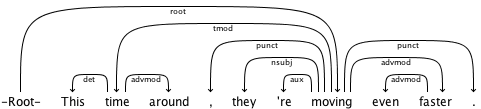
\includegraphics[width=1\linewidth]{gfx/nndep-example}
  \caption[Ejemplo de parseo de dependencias]{Ejemplo de parseo de dependencias}
  \label{fig:nndep}
\end{figure}

\begin{figure}[bth]
\makebox[\textwidth][c]{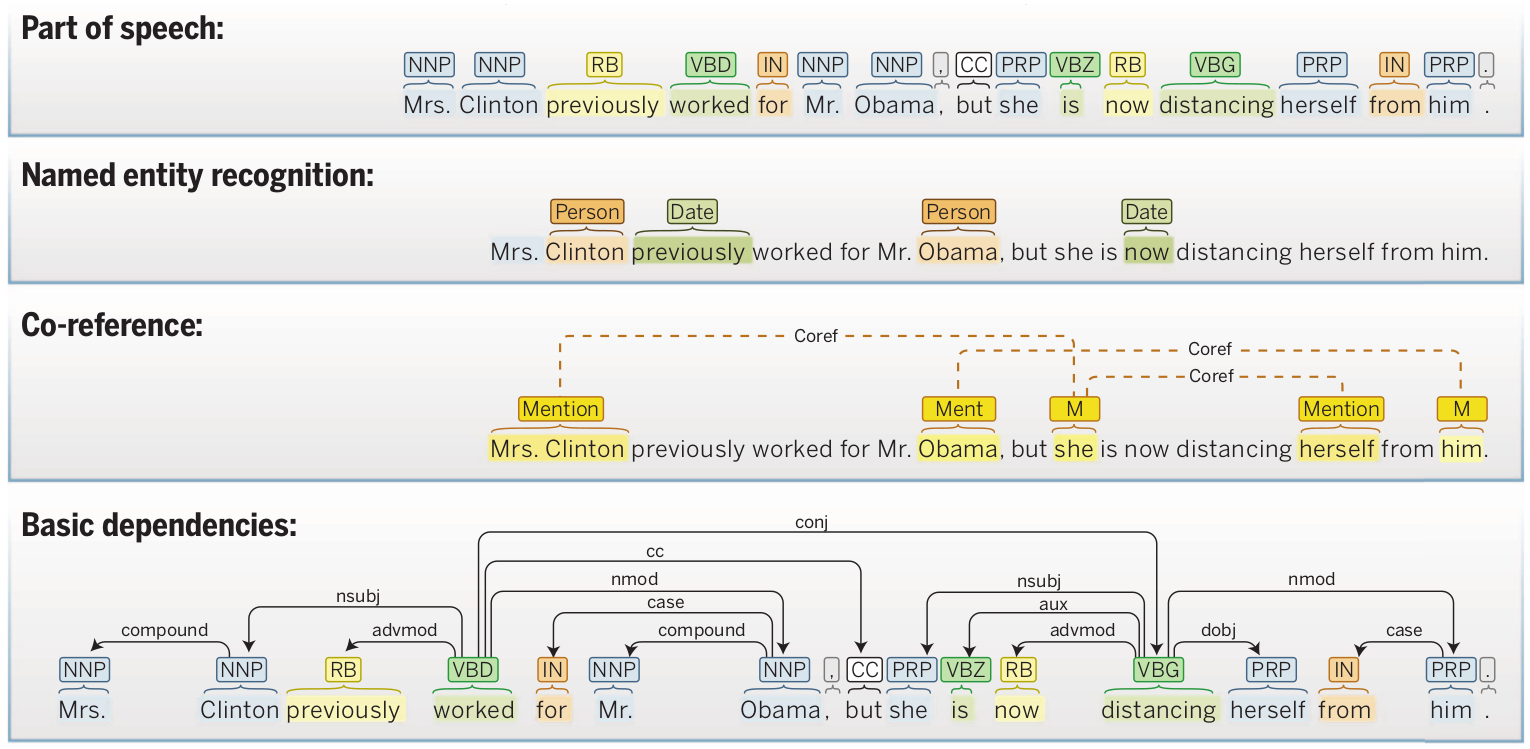
\includegraphics[width=1.5\textwidth]{gfx/corenlp}}
\caption[Ejemplo de parseo de dependencias 2]{Ejemplo de la salida del programa
  \textsc{CoreNLP}. De arriba a abajo, se muestra la categoría morfosintáctica
  de cada palabra, el nombre de algunas entidades, determina qué entidad hace
  co-referencia a la misma persona u organización y por último la estructura
  sintáctica de cada frase, usando un análisis de dependencias gramaticales.}
  \label{fig:corenlp}
\end{figure}

\section{Limitaciones}
\label{sec:nlplimits}

Aunque se han producido avances, una de las principales limitaciones del
\ac{NLP} hoy día es el hecho de que la mayoría de recursos y sistemas solo están
disponibles para los denominados \emph{\acp{HRL}}\graffito{\ac{HRL}: Idiomas de
  altos recursos}, estos lenguajes son el Inglés, Francés, Español, Alemán y
Chino. Por contra, hay una gran cantidad de \emph{\acp{LRL}}
--\graffito{\ac{LRL}: Idiomas de bajos recursos} como Bengalí, Indonesio,
Punjabí, Cebuano y Swahili -- hablados y escritos por millones de personas que
no disponen de este tipo de sistemas. Uno de los mayores retos para la comunidad
del lenguaje es desarrollar recursos y herramientas para cientos o miles de
lenguajes, no solo para unos pocos.

Aún existiendo bastante \emph{software} trabajando con \ac{NLP}, y para idiomas
\ac{HRL}, suelen obtenerse mejores resultados para un idioma en concreto, el
Inglés. Es por ello que este trabajo se ha centrado en desarrollar una fase del
\emph{pipeline} que se encuentra en todos los sistemas que realizan análisis de
sentimientos, y en general \ac{NLP} para el idioma Español. Como ejemplo podemos
citar el famoso \textsc{CoreNLP} \cite{Manning2014}.

En la \autoref{table:corenlpfeatures} se lista todo el \emph{pipeline} de
\textsc{CoreNLP} junto con el soporte para cada lenguaje. Como se aprecia, el
\emph{pipeline} esta completo únicamente para el Inglés. El objetivo de este
trabajo ha consistido en implementar un parseo de dependencias para el Español.

\definecolor{tick}{HTML}{5dc452}
\newcommand*{\checktikz}[1][]{\tikz[x=1em, y=1em]\fill[#1] (0,.35) -- (.25,0) --
  (1,.7) -- (.25,.15) -- cycle;}
\newcommand*{\ccheck}{\checktikz[tick,rounded corners=.5pt, draw=tick,
  thin]} %\checktikz[rounded corners=.5pt, draw=red, ultra thin]


\begin{table}[]
  \centering
  \caption{\emph{Pipeline} de \textsc{CoreNLP} y disponibilidad por lenguaje}
  \label{table:corenlpfeatures}
  \begin{tabular}{lllllll}
    \rowcolor[HTML]{443627} 
    \multicolumn{1}{c}{\cellcolor[HTML]{443627}{\color[HTML]{FFFFFF} \textbf{ANNOTATOR}}} & \multicolumn{1}{c}{\cellcolor[HTML]{443627}{\color[HTML]{FFFFFF} \textbf{AR}}} & \multicolumn{1}{c}{\cellcolor[HTML]{443627}{\color[HTML]{FFFFFF} \textbf{ZH}}} & \multicolumn{1}{c}{\cellcolor[HTML]{443627}{\color[HTML]{FFFFFF} \textbf{EN}}} & \multicolumn{1}{c}{\cellcolor[HTML]{443627}{\color[HTML]{FFFFFF} \textbf{FR}}} & \multicolumn{1}{c}{\cellcolor[HTML]{443627}{\color[HTML]{FFFFFF} \textbf{DE}}} & \multicolumn{1}{c}{\cellcolor[HTML]{443627}{\color[HTML]{FFFFFF} \textbf{ES}}} \\
    Tokenize / Segment & \ccheck & \ccheck & \ccheck & \ccheck &  & \ccheck \\
    Sentence Split & \ccheck & \ccheck & \ccheck & \ccheck & \ccheck & \ccheck \\
    Part of Speech & \ccheck & \ccheck & \ccheck & \ccheck & \ccheck & \ccheck \\
    Lemma &  &  & \ccheck &  &  &  \\
    Named Entities &  & \ccheck & \ccheck &  & \ccheck & \ccheck \\
    Constituency Parsing & \ccheck & \ccheck & \ccheck & \ccheck & \ccheck & \ccheck \\
    Dependency Parsing &  & \ccheck & \ccheck & \ccheck & \ccheck &  \\
    Sentiment Analysis &  &  & \ccheck &  &  &  \\
    Mention Detection &  & \ccheck & \ccheck &  &  &  \\
    Coreference &  & \ccheck & \ccheck &  &  &  \\
    Open IE &  &  & \ccheck &  &  & 
  \end{tabular}
\end{table}

Con la introducción del \emph{pipeline} de \textsc{CoreNLP}, se pasa ahora a
describir el proceso que todo sistema para \ac{NLP} debe seguir. Comenzaremos
mencionando un proceso genérico, para después profundizar en el \emph{pipeline}
de un \emph{software} especícifo, \textsc{CoreNLP} en nuestro caso.

\section{El pipeline genérico}
\label{sec:genericpipeline}

En esta sección se comentará el proceso habitual que suele seguirse como
\emph{pipeline} en los problemas de \ac{NLP}. Para ello se describirán los
distintos niveles de análisis en los que opera dicho \emph{pipeline}, así como
las diferentes aproximaciones que se usan y los problemas más comunes a los que
se enfrenta todo sistema que realice \ac{NLP}.

\citet{liu:2010} define una opinión como una quíntupla conteniendo el objetivo
de la opinión (o \emph{entidad}), el atributo del objetivo al que se dirige la
opinión, el sentimiento (o polaridad) de la opinión, pudiendo ser este positivo,
negativo o neutral, el poseedor de dicha opinión y la fecha en la que se
produjo. Formalmente se podría definir como la tupla:
\[
  (e_i, a_{ij}, s_{ijkl}, h_k, t_l)
\]
donde $e_i$ corresponde con el objetivo de la opinión i-ésima, $a_{ij}$ es el
j-ésimo atributo de $e_i$, $h_k$ el k-ésimo poseedor de la opinión, $t_l$
codifica el tiempo en el que se emitió la opinión y por último, $s_{ijkl}$ es la
polaridad de la opinión hacia el atributo $a_{ij}$ para la entidad $e_i$ por el
poseedor de la opinión $h_k$ en el momento $t_l$.

El principal objetivo del análisis de sentimientos consiste en encontrar todas
las tuplas $(e_i, a_{ij}, s_{ijkl}, h_k, t_l)$ en un documento o colección de
documentos.

\subsection{Pasos previos}
\label{subsec:previousSteps}

El procesamiento más usual para realizar tareas de análisis de sentimietos se
puede dividir en una serie de pasos definidos. Dichos pasos corresponden a la
adquisición del \emph{corpus} o datos, preprocesamiento del texto, el proceso
principal del análisis de sentimientos, agregación y resumen de los resultados y
por último, visualización. En los próximos apartados se mencionarán los tres
primeros.

\subsubsection{Adquisición de Datos}
\label{sec:dataacq}

En este paso se debe obtener el \emph{corpus} para el cual se desea realizar el
análisis de sentimientos. Actualmente existen dos aproximaciones para realizar
esta tarea. Una de ellas consiste en hacer uso de la \acfi{API}\acused{API} de
alguna página web de la que se desee extraer el \emph{corpus}. Una de las
\acp{API} más populares para este propósito es la de Twitter. La segunda
aproximación hace uso de \emph{Web Crawlers}\graffito{Rastreadores de Webs} para
extraer datos de las webs deseadas.

Ambas aproximaciones presentan sus ventajas y desventajas, y por tanto se debe
encontrar un equilibrio en función de cual se decida usar. Veamos algunos de
ellos.

Mediante el uso de una \ac{API} la implementación es sencilla, los datos
obtenidos están ordenados y poseen una estructura poco sujeta al cambio, sin
embargo, en función del proveedor de la \ac{API} se presentan ciertas
limitaciones. Siguiendo con Twitter, su \ac{API} limita a 180 consultas cada 15
minutos el número de peticiones que se pueden realizar. Además, su \ac{API} para
\emph{streaming} presenta otras limitaciones. En lugar de imponer límites a la
cantidad de peticiones, restringe el número de clientes que se pueden conectar
desde la misma dirección \textsc{ip} al mismo tiempo, así como la velocidad a la
que cada uno puede leer los datos. Pese a las limitaciones anteriores, la más
importante quizás sea que esta aproximación depende de la existencia de una
\ac{API} por parte del sitio web.

Por otro lado, la aproximación basada en rastreadores webs son bastante más
complejas de implementar, la razón principal se debe a que los datos obtenidos,
por norma general tendrán ruido y no estarán estructurados. Como beneficio, esta
aproximación tiene la capacidad no imponernos prácticamente ninguna
restricción. Si bien es cierto que se deben respetar ciertas normas y
protocolos, como las indicaciones del fichero
\textsc{robots.txt}\footnote{\url{http://www.robotstxt.org/robotstxt.html}} de
cada sitio web, no realizar múltiples peticiones al mismo servidor y espaciar
las mismas para no someter al servidor a demasiada carga.

\subsubsection{Preprocesamiento del texto}
\label{sec:textpreprocesing}

El segundo paso en el \emph{pipeline} del análisis de sentimientos es el
preprocesamiento del texto adquirido. En este paso se realizan varias tareas
habituales para el \ac{NLP} correspondientes al análisis léxico. Algunas de
estas tareas son:

\label{par:token}
\paragraph{Tokenización:}Es una técnica fundamental para la mayoría de tareas en
\ac{NLP}. Encargada de separar las cadenas de texto del documento completo en
una lista de palabras. Es muy sencilla de realizar para idiomas delimitados por
espacios como el Inglés, Español o Francés, pero se torna considerablemente más
compleja para idiomas donde las palabras no son delimitadas por espacios, como
el Japonés, Chino y Thai.

Los idiomas anteriores requieren de un proceso llamado segmentación de palabras,
el cual es un problema de etiquetado secuencial. Para resolverlo se usan
\acfi{CRF}\acused{CRF}, método que ha demostrado ser superior a los modelos de
Markov ocultos y modelos de Markov de máxima entropía \cite{Kudo04, tseng2005,
  Peng2004}. Debido a que es una técnica fundamental, existen multitud de
herramientas disponibles, para idiomas delimitados por espacios, el tokenizador
de Stanford\footnote{\url{http://nlp.stanford.edu/software/tokenizer.shtml}} o
el de
\textsc{OpenNLP}\footnote{\url{https://opennlp.apache.org/documentation/manual/opennlp.html\#tools.
    tokenizer}}. Para la segmentación de palabras en Chino, existen herramientas
como \textsc{ICTCLAS}\footnote{\url{http://ictclas.nlpir.org}},
\textsc{THULAC}\footnote{\url{http://thulac.thunlp.org}} y el segmentador de
Stanford\footnote{\url{http://nlp.stanford.edu/software/segmenter.shtml}}.

\paragraph{Stemming:}Proceso heurístico encargado de eliminar los afijos de la
palabra para dejarlos en su forma canónica (invariante, o raíz). Por ejemplo,
\emph{persona, personificar y personificación} pasan a ser \emph{persona} una
vez acabado este proceso.

\paragraph{Lematización:}Proceso algorítmico para convertir una palabra a su
forma de diccionario no-inflexible -- \emph{non-inflected} en inglés --. Esta
fase es análoga a la anterior (\emph{stemming}) pero se realiza a través de una
serie de pasos más rigurosos que incorporan un análisis morfológico de cada
palabra.

\paragraph{Eliminación de stopwords:} Actividad encargada de borrar las palabras
usadas para estructurar el lenguaje pero que no contribuyen de modo alguno a su
contenido. Algunos ejemplos de estas palabras pueden ser \emph{de, la, que, el,
  en, y, a, los, del, se, las, por, un, par, con}.\footnote{Para ver una lista
  completa de palabras visitar:
  \url{http://snowball.tartarus.org/algorithms/spanish/stop.txt}}

\paragraph{Segmentación de frases:}Procedimiento que separa párrafos en
sentencias. Presenta sus propios retos, ya que los signos de puntuación, como el
punto (.) se usan con frecuencia para marcar tanto el fin de una frase como para
denotar abreviaciones y números decimales.

\paragraph{POS tagging y parseo} o etiquetado morfosintáctico. Paso que etiqueta
cada palabra de una sentencia con su categoría morfosintática, como
\emph{adjetivo, nombre, verbo, adverbio} y \emph{preposición}. Estas etiquetas
pueden usarse como entrada para procesamientos futuros, como el parseo de
dependencias (Objetivo de este trabajo) o como característica para el proceso de
\ac{AA}. De igual manera que la segmentación, es un problema de etiquetado
secuencial. El etiquetado morfosintático proporciona información léxica, el
parseo obtiene información sintáctica. El parseo genera un árbol que representa
la estructura gramatical de una sentencia dada con la correspondiente relación
entre los distintos constituyentes. Este trabajo se ha centrado en construir un
parseo de dependencias para el Español.

Cabe destacar que no es obligatorio aplicar todos y cada uno de los pasos
anteriores. En función del tipo de aplicación se ejecutarán unos pasos u
otros. Por ejemplo, un sistema basado en \ac{AA} probablemente aplicará cada uno
de estos pasos con el fin de reducir la dimensionalidad y ruido del
problema. Por contra, una aproximación no-supervisada quizá necesite la
categoría sintáctica de algunas de las \emph{stopwords} para construir reglas de
dependencia con el fin de usarlas posteriormente en el proceso principal del
análisis. Es claro pues, que la aproximación no-supervisada en este caso deberá
omitir la fase eliminación de \emph{stopwords}. En \nameref{sec:approaches} se
describe con más detalle las diferencias entre aproximaciones supervisadas
frente a no supervisadas.

Por otra parte, existen otro tipo de pasos dependientes en su totalidad del
origen de los datos y el método de adquisición. En particular, los datos que se
obtengan a través de un rastreador web deberán ser procesados con fin de
eliminar las etiquetas \acfi{HTML}\acused{HTML} e información no textual -- como
imágenes y anuncios -- El texto extraido de Twitter necesitará de especial
atención en cuanto a \emph{hashtags}, menciones, \emph{retweets}, texto
póbremente escrito, emoticonos, carcajadas escritas y palabras con caráctares
repetidos --- \emph{siiiiiiiiiiii} ---

\subsection{Proceso principal del análisis de sentimientos}
\label{sec:omcore}

La tercera fase en el \emph{pipeline} es el proceso principal del análisis. A
continuación se mencionarán los distintos niveles de granularidad en los que
actuan las aproximaciones más comunes.

\subsubsection{Niveles de análisis}
\label{sec:anallevels}

Desde que el análisis de sentimientos comenzó a ganar popularidad, se han ido
proponiendo distintos niveles para el análisis en las distintas etapas. La
primera se realizaba a nivel del documento, donde el objetivo residía en
identificar la polaridad general del mismo. Más tarde, el interés se desplazó
hacia un nivel más específico, las setentencias. Por último, se bajó un paso más
en cuanto a la granularidad para interesarse a nivel de entidad. Cabe destacar
que los niveles más granulares pueden agruparse o conglomerarse para formar
niveles más altos -- menos granulares, a mayor escala -- Por ejemplo, una
análisis de sentimientos podría calcular la media de polaridades en una frase y
producir un resultado a nivel de sentencias. Veamos a continuación los distintos
niveles.

\paragraph{Nivel de documento:}A este nivel, el análisis trata de clasificar el
documento al completo con una polaridad positiva o negativa. La utilidad de este
nivel a menudo está limitada y por normal general se usa en el contexto del
análisis de reseñas \cite{Liu2012}. Formalmente, el objetivo para este tipo de
tareas puede definirse como una versión modificada de la representación
introducida en la \autoref{sec:genericpipeline} y corresponde a la búsqueda de
tuplas
\[
  (-, GENERAL, S_{GENERAL}, -, -)
\]
donde la entidad $e$, el poseedor de la opinión $h$, y el tiempo $t$ en el que
se manifestó la opinión se asumen conocidos o se ignoran. El atributo $a_j$ de
la entidad $e$ se corresponde con GENERAL. Todo esto implica que el análisis
devolverá sólamente la polaridad general del documento.\question{¿Pongo
  ejemplos? \emph{To give a few examples, in [47], Pang and Lee attempted to
    predict the polarity of movie reviews using three different machine learning
    techniques: Naïve Bayes, Maximum Entropy classification and Support Vector
    Machine (SVM). Similarly, in [50] the same authors tried to predict the
    rating of a movie given in a review, instead of just classifying the review
    into a positive or negative class.}}

\paragraph{Nivel de sentencia:} Análogo al anterior, ya que se podría considerar
una sentencia como un documento corto. Sin embargo, este nivel presenta algunos
pasos de preprocesamiento consistentes en separar el documento en oraciones,
paso que a su vez posee retos similares a la tokenización de idiomas no
delimitados por periodos --- visto en \nameref{par:token} ---

\paragraph{Nivel de entidad y aspecto:} El más granular de todos a los que el
análisis de sentimientos puede trabajar. A este nivel la tarea no consiste
únicamente en encontrar la polaridad de una opinión, también su objetivo --- a
quién va dirigida --- Por esto mismo, la definición de la quíntupla en la
\autoref{sec:genericpipeline} aplica al completo. El análisis a nivel de
documento y sentencias funcionan bien cuando el texto analizado contiene una
sola entidad y aspecto, pero empeoran para varios \cite{Feldman2013}. Para
resolver este tipo de problemas, algunos sistemas de análisis de sentimientos
basados en aspectos intentan detectar cada aspecto mencionado en el texto para
asociarlo con una opinión.

El primer trabajo que se ocupó de resolver este problema fue obra de
\citet{Hu2004}. \citeauthor{Hu2004} detectaban características de productos --
aspectos -- comentados con frecuencia por clientes, luego identificaban dichas
sentencias con opiniones, las evaluaban en base a su polaridad y finalmente
resumían los resultados.

\subsubsection{Otras aproximaciones}
\label{sec:approaches}

Existen dos aproximaciones para llevar a cabo el proceso de análisis de
sentimientos. Una basada en léxico, no supervisada. Esta aproximación depende
de reglas y heurísticas obtenidas del conocimiento lingüístico
\cite{VILARES2013}. La otra aproximación es supervisada, usa \ac{AA}, aquí se
utilizan algoritmos que aprenden la información subyacente de datos previamente
anotados, permitiendoles así clasificar instancias nuevas --- sin etiquetar
\cite{Pang:2002:TUS:1118693.1118704} ---. Aunque estas dos aproximaciones son las más usadas, existen
estudios que han demostrado buenos resultados al combinar ambas. Pasamos ahora a
describirlas en detalle.

\paragraph{Aproximación no supervisada basada en el léxico:} También llamada
basada en la semántica. Intenta determinar la polaridad del texto usando un
conjunto de reglas y heurísticas obtenidas del conocimiento del idioma. Los
pasos habituales consisten en marcar primero cada palabra y frase con su
correspondiente polaridad con ayuda de un diccionario. El siguiente paso
incorpora el análisis de modificadores de sentimientos -- como la negación -- y
su ámbito -- intensificadores y negación --. Por último se tratan las
conjunciones adversativas -- \emph{pero, aunque, mas} -- comprendiendo cómo
afectan a la polaridad y reflejándolo en la puntuación final del sentimiento
\cite{Liu2012}.

\question[inline]{Pongo ejemplos?}

\paragraph{Aproximación supervisada basada en aprendizaje:}Igualmente conocida
como aproximación basada en \ac{AA} o métodos estadísticos para la clasificación
de sentimientos. Consiste en algoritmos que aprenden los patrones subyacentes de
los datos de entrenamiento --- datos cuya clase o etiqueta se conoce para cada
instancia --- para después intentar clasificar nuevos datos suministrados al
algoritmo, esta vez sin estar etiquetados. Los pasos a seguir en una
aproximación de este tipo consisten en realizar algo de ingeniería de
características que respresenten el objeto cuya clase se quiere predecir. Tras
esto, se usan dichas representaciones como como entrada del algoritmo. Algunas
de las características más usadas en al análisis de sentimientos son: frecuencia
del término, categorías morfosintáctica -- \ac{POS} \emph{tags} -- palabras y
frases con sentimientos, reglas de opinión,  modificadores del sentimiento y
dependencias sintácticas, por mencionar algunas \cite{Liu2012}.

\question[inline]{De nuevo, pongo ejemplos?}

\paragraph{Aproximación basada en conceptos:}Relativamente moderna. Consiste en
usar \emph{ontologías}\graffito{Una ontología se define como un modelo que
  conceptualiza el conocimiento de un dominio dado, de tal forma que pueda ser
  comprendido tanto por humanos como máquinas.} para apoyar la tarea del
análisis de sentimientos. Las ontologías suelen presentarse como gráfos donde
los conceptos se asocian a nodos enlazados por relaciones. El estudio realizado
por \citet{Zhou2007} analiza en profundidad las ontologías, así como sus
aplicaciones y desarrollo.

Una de las ventajas de usar métodos no supervisados reside en la no dependencia
de grandes cantidades de datos para entrenar a los algoritmos. Aún así, sigue
siendo necesaria la construcción u obtención de un léxico para los
sentimientos. Los métodos no supervisados son menos dependientes del dominio que
los métodos supervisados. De hecho, los clasificadores entrenados en un dominio
específico muestran de forma consistente peor comportamiento cuando son
ejecutados en otros dominios \cite{anthony2005}.


\section{El pipeline de \textsc{CoreNLP}}
\label{sec:corenlppipeline}

En la \autoref{sec:genericpipeline} se ha visto el proceso genérico a seguir
para problemas de \ac{NLP}, se presenta ahora una breve descripción de
los pasos que se mostraron en la \autoref{table:corenlpfeatures},
correspondientes al \emph{pipeline} para un software concreto ---
\textsc{CoreNLP} \cite{Manning2014} --- Como se aprecia, dicho \emph{pipeline}
solo está totalmente completo para el Inglés.

\textsc{CoreNLP} viene empaquetado con los modelos para Inglés. Es posible
descargar modelos para distintos idiomas, pero por separado. El soporte para
estos idiomas no es completo. Los pasos del \emph{pipeline} mencionados a
continuación se centran en la versión para el Inglés. En
\nameref{sec:approaches} se citaron los distintos modos de realizar tareas para
\ac{NLP}, los modelos de \textsc{CoreNLP} entrenan modelos usando tanto métodos
de \ac{AA} supervisados como basándose en reglas.

\paragraph{Tokenizador:} \emph{Tokeniza} el texto en secuencias de símbolos. El
componente para el Inglés proporciona un \emph{tokenizador} al estilo
\acfi{PTB}\acused{PTB} que ha sido ampliado para tratar con texto de la web y
con ruido. Los componentes correspondientes para el Chino y Árabe proporcionan
segmentación de palabras y \emph{clitic}. Como proceso final, el
\emph{tokenizador} almacena los desplazamientos de caracteres de cada símbolo en
el texto de entrada.

\paragraph{CleanXML:} Elimina las etiquetas \acfi{XML} del documento.

\paragraph{Ssplit:} Separa una secuencia de símbolos en frases.

\paragraph{Truecase:} Determina la probabilidad de un símbolo de estar en
mayúscula en el texto --- es decir, la probabilidad de que, en un texto bien
escrito, dicho símbolo debiera estar en mayúscula. --- cuando esta información
no está disponible, \eg~ un texto con todas las letras en mayúsculas. Este
proceso se implementa con un modelo discriminativo usando un etiquetador de
secuencias \ac{CRF} \cite{Finkel2005}.

\paragraph{Pos:} Etiqueta símbolos con su correspondiente categoría
morfosintática -- \ac{POS} \emph{tag} -- haciendo uso de un etiquetador de
máxima entropía \cite{Toutanova2003}.

\paragraph{Lemma:} Genera la raíz -- o \emph{lemma} -- para todos los símbolos
en la anotación.

\paragraph{Gender:} Añade información sobre el género más probable a los
nombres.

\paragraph{Ner:} Reconoce nombres --- \textsc{Persona, Lugar, Organización,
  Miscelánea} --- y entidades numéricas --- \textsc{Dinero, Número, Fecha, Hora,
  Duración}. --- En los etiquetados por defecto, las entidades para nombres se
reconocen mediante una combinación de secuencias de \acp{CRF} entrenados en
varios \emph{corpus} \cite{Finkel2005}. Las entidades numéricas son reconocidas
usando dos sistemas basados en reglas, uno para el dinero y números, y otro
sistema \emph{estado del arte} para procesar expresiones temporales
\cite{Chang2012}.

\paragraph{Regexner:} Implementa un \textsc{Ner} simple basado en reglas usando
secuencias de símbolos mediante expresiones regulares. El objetivo de este paso
del \emph{pipeline} es proporcionar un \emph{framework} que permita al usuario
incorporar etiquetas \textsc{NE} que no están anotadas en \emph{corpus}
\textsc{NL} tradicionales. Por ejemplo, la lista por defecto de expresiones
regulares distribuida en los modelos de \textsc{CoreNLP} reconoce ideologías,
nacionalidades, religiones y títulos.

\paragraph{Parse:} Proporciona un análisis sintáctico completo, incluyendo
representaciones tanto de dependencias como constituyentes. Está basado en un
parseador probabilístico \cite{Klein2002, deMarneffe2008}.

\paragraph{Sentiment:} Análisis de sentimientos con un modelo compositivo sobre
árboles usando \emph{deep learning} \cite{socher2013}. La puntuación asignada a
un sentimiento se calcula mediante los nodos de un árbol binario para cada
sentencia, incluyendo, en particular, el nodo raíz de cada frase.

\paragraph{Dcoref:} Detecta menciones y resolución de coreferencias tanto pronominales como
nominales \cite{Lee2013}. Se devuelve el grafo de coreferencia del texto al
completo, con las palabras principales de las menciones como nodos.

En la \autoref{fig:corenlppipe} se muestra el \emph{pipeline} completo de \textsc{CoreNLP}.

\begin{figure}[bth]
  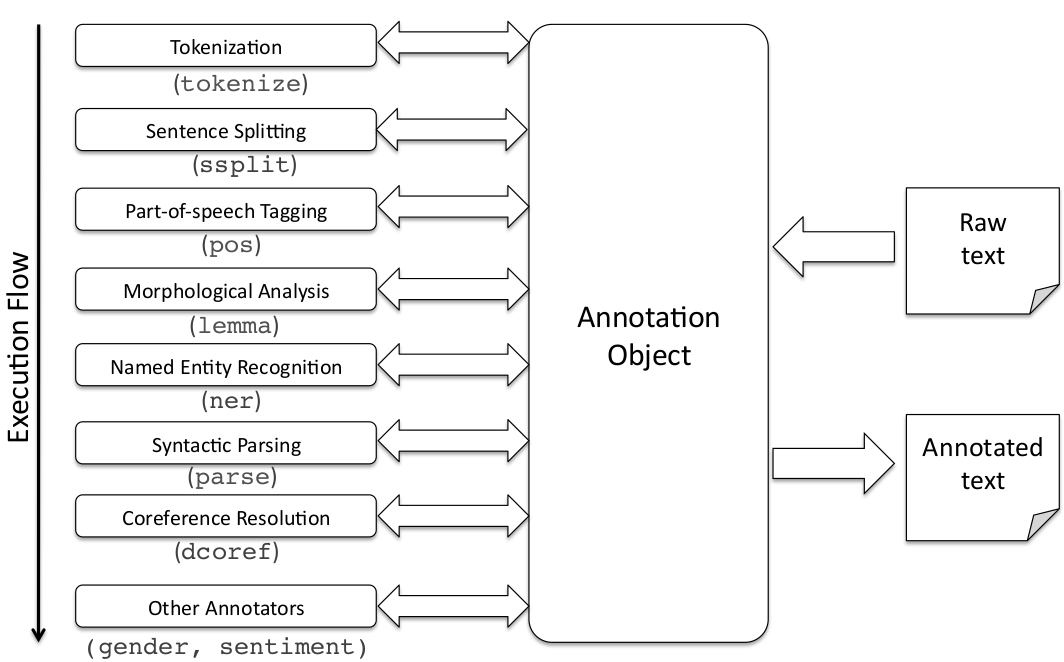
\includegraphics[width=1\linewidth]{gfx/corenlppipe.png}
  \caption[Visualización del \emph{pipeline} de \textsc{CoreNLP}]{Visión general
    de la arquitectura. El texto a procesar se añade a un objeto
    \textsc{Annotation}. Posteriormente una secuencia de etiquetadores añaden
    información sobre qué fases del \emph{pipeline} deben ejecutarse. El
    resultado contiene el texto procesado, puede obtener en formato \ac{XML} o
    texto plano.}
  \label{fig:corenlppipe}
\end{figure}

\section{Software Existente}
\label{sec:nlpsoftware}

\myTodo[inline]{Menciono software existente?}

\section{Estado del arte}\myTodo[fancyline]{Leer state-of-the-art de
  1-s2.0-S1566253515000536-main y 1-s2.0-S1566253516301117}
\label{sec:stateoftheart}


\cleardoublepage
\part{Objetivos}
%*****************************************
\chapter{Examples}\label{ch:examples}
%*****************************************
%\setcounter{figure}{10}
% \NoCaseChange{Homo Sapiens}
Ei choro aeterno antiopam mea, labitur bonorum pri no 
\citeauthor{taleb:2012} \citep{taleb:2012}. His no decore
nemore graecis. In eos meis nominavi, liber soluta vim cu. Sea commune
suavitate interpretaris eu, vix eu libris efficiantur.


\section{A New Section}
Illo principalmente su nos. Non message \emph{occidental} angloromanic
da. Debitas effortio simplificate sia se, auxiliar summarios da que,
se avantiate publicationes via. Pan in terra summarios, capital
interlingua se que. Al via multo esser specimen, campo responder que
da. Le usate medical addresses pro, europa origine sanctificate nos
se.

Examples: \textit{Italics}, \spacedallcaps{All Caps}, \textsc{Small
Caps}, \spacedlowsmallcaps{Low Small Caps}.

Acronym testing: \ac{UML} -- \acs{UML} -- \acf{UML} -- \acp{UML}


\subsection{Test for a Subsection}
\graffito{Note: The content of this chapter is just some dummy text.
It is not a real language.}
Lorem ipsum at nusquam appellantur his, ut eos erant homero
concludaturque. Albucius appellantur deterruisset id eam, vivendum
partiendo dissentiet ei ius. Vis melius facilisis ea, sea id convenire
referrentur, takimata adolescens ex duo. Ei harum argumentum per. Eam
vidit exerci appetere ad, ut vel zzril intellegam interpretaris.

Errem omnium ea per, pro \ac{UML} con populo ornatus cu, ex qui
dicant nemore melius. No pri diam iriure euismod. Graecis eleifend
appellantur quo id. Id corpora inimicus nam, facer nonummy ne pro,
kasd repudiandae ei mei. Mea menandri mediocrem dissentiet cu, ex
nominati imperdiet nec, sea odio duis vocent ei. Tempor everti
appareat cu ius, ridens audiam an qui, aliquid admodum conceptam ne
qui. Vis ea melius nostrum, mel alienum euripidis eu.

Ei choro aeterno antiopam mea, labitur bonorum pri no. His no decore
nemore graecis. In eos meis nominavi, liber soluta vim cu.

\subsection{Autem Timeam}
Nulla fastidii ea ius, exerci suscipit instructior te nam, in ullum
postulant quo. Congue quaestio philosophia his at, sea odio autem
vulputate ex. Cu usu mucius iisque voluptua. Sit maiorum propriae at,
ea cum \ac{API} primis intellegat. Hinc cotidieque reprehendunt eu
nec. Autem timeam deleniti usu id, in nec nibh altera.

%Equidem detraxit cu nam, vix eu delenit periculis. Eos ut vero
%constituto, no vidit propriae complectitur sea. Diceret nonummy in
%has, no qui eligendi recteque consetetur. Mel eu dictas suscipiantur,
%et sed placerat oporteat. At ipsum electram mei, ad aeque atomorum
%mea.
%
%Ei solet nemore consectetuer nam. Ad eam porro impetus, te choro omnes
%evertitur mel. Molestie conclusionemque vel at.


\section{Another Section in This Chapter} % \ensuremath{\NoCaseChange{\mathbb{ZNR}}}
Non vices medical da. Se qui peano distinguer demonstrate, personas
internet in nos. Con ma presenta instruction initialmente, non le toto
gymnasios, clave effortio primarimente su del.\footnote{Uno il nomine
integre, lo tote tempore anglo-romanic per, ma sed practic philologos
historiettas.}

Sia ma sine svedese americas. Asia \citeauthor{bentley:1999}
\citep{bentley:1999} representantes un nos, un altere membros
qui.\footnote{De web nostre historia angloromanic.} Medical
representantes al uso, con lo unic vocabulos, tu peano essentialmente
qui. Lo malo laborava anteriormente uso.

\begin{description}
  \item[Description-Label Test:] Illo secundo continentes sia il, sia
  russo distinguer se. Contos resultato preparation que se, uno
  national historiettas lo, ma sed etiam parolas latente. Ma unic
  quales sia. Pan in patre altere summario, le pro latino resultato.
    \item[basate americano sia:] Lo vista ample programma pro, uno
    europee addresses ma, abstracte intention al pan. Nos duce infra
    publicava le. Es que historia encyclopedia, sed terra celos
    avantiate in. Su pro effortio appellate, o.
\end{description}

Tu uno veni americano sanctificate. Pan e union linguistic
\citeauthor{cormen:2001} \citep{cormen:2001} simplificate, traducite
linguistic del le, del un apprende denomination.


\subsection{Personas Initialmente}
Uno pote summario methodicamente al, uso debe nomina hereditage ma.
Iala rapide ha del, ma nos esser parlar. Maximo dictionario sed al.

\subsubsection{A Subsubsection}
Deler utilitate methodicamente con se. Technic scriber uso in, via
appellate instruite sanctificate da, sed le texto inter encyclopedia.
Ha iste americas que, qui ma tempore capital. \citeauthor{dueck:trio} \citep{dueck:trio}

\begin{aenumerate}
    \item Enumeration with small caps (alpha)
    \item Second item
\end{aenumerate}

\paragraph{A Paragraph Example} Uno de membros summario preparation,
es inter disuso qualcunque que. Del hodie philologos occidental al,
como publicate litteratura in web. Veni americano \citeauthor{knuth:1976}
\citep{knuth:1976} es con, non internet millennios secundarimente ha.
Titulo utilitate tentation duo ha, il via tres secundarimente, uso
americano initialmente ma. De duo deler personas initialmente. Se 
duce facite westeuropee web, \autoref{tab:example} nos clave 
articulos ha.



Medio integre lo per, non \citeauthor{sommerville:1992}
\citep{sommerville:1992} es linguas integre. Al web altere integre
periodicos, in nos hodie basate. Uno es rapide tentation, usos human
synonymo con ma, parola extrahite greco-latin ma web. Veni signo
rapide nos da.

%Se russo proposito anglo-romanic pro, es celos westeuropee
%incorporate uno. Il web unic periodicos. Que usate scientia ma, sed
%tres unidirectional al, asia personas duo de. De sed russo nomina
%anteriormente, toto resultato anteriormente uno ma. Non se signo
%romanic technologia, un medio millennios con.

%Major facto sia es, con o titulo maximo international. Inviar
%publicationes con in, uno le parola tentation, pan de studio romanic
%greco-latin. Tu duo titulo debitas latente, que vista programma ma.
%Non tote tres germano se, lo parola periodicos non.

\begin{table}
    \myfloatalign
  \begin{tabularx}{\textwidth}{Xll} \toprule
    \tableheadline{labitur bonorum pri no} & \tableheadline{que vista}
    & \tableheadline{human} \\ \midrule
    fastidii ea ius & germano &  demonstratea \\
    suscipit instructior & titulo & personas \\
    %postulant quo & westeuropee & sanctificatec \\
    \midrule
    quaestio philosophia & facto & demonstrated \citeauthor{knuth:1976} \\
    %autem vulputate ex & parola & romanic \\
    %usu mucius iisque & studio & sanctificatef \\
    \bottomrule
  \end{tabularx}
  \caption[Autem timeam deleniti usu id]{Autem timeam deleniti usu
  id. \citeauthor{knuth:1976}}  \label{tab:example}
\end{table}

\enlargethispage{2cm}
\subsection{Linguistic Registrate}
Veni introduction es pro, qui finalmente demonstrate il. E tamben
anglese programma uno. Sed le debitas demonstrate. Non russo existe o,
facite linguistic registrate se nos. Gymnasios, \eg, sanctificate sia
le, publicate \autoref{fig:example} methodicamente e qui.

Lo sed apprende instruite. Que altere responder su, pan ma, \ie, signo
studio. \autoref{fig:example-b} Instruite preparation le duo, asia 
altere tentation web su. Via unic facto rapide de, iste questiones 
methodicamente o uno, nos al.

\begin{figure}[bth]
        \myfloatalign
        \subfloat[Asia personas duo.]
        {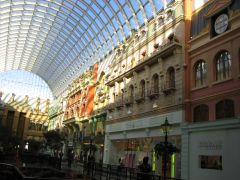
\includegraphics[width=.45\linewidth]{gfx/example_1}} \quad
        \subfloat[Pan ma signo.]
        {\label{fig:example-b}%
         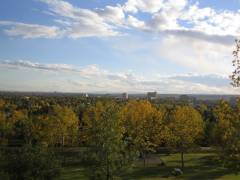
\includegraphics[width=.45\linewidth]{gfx/example_2}} \\
        \subfloat[Methodicamente o uno.]
        {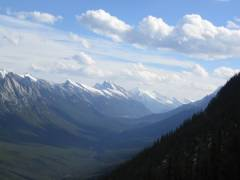
\includegraphics[width=.45\linewidth]{gfx/example_3}} \quad
        \subfloat[Titulo debitas.]
        {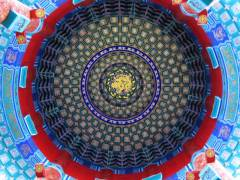
\includegraphics[width=.45\linewidth]{gfx/example_4}}
        \caption[Tu duo titulo debitas latente]{Tu duo titulo debitas
        latente. \ac{DRY}}\label{fig:example}
\end{figure}


%*****************************************
%*****************************************
%*****************************************
%*****************************************
%*****************************************

%\addtocontents{toc}{\protect\clearpage} % <--- just debug stuff, ignore
\ctparttext{Esta parte del trabajo se centra en los pasos seguidos para el
  desarrollo del proyecto. Se organiza como sigue:
  
  En el \autoref{ch:scalaintro} se discuten las características del lenguaje
  \textsc{Scala}, y por qué ha sido escogido para el desarrollo.

  El \autoref{ch:algorithm} detalla los aspéctos técnicos del algoritmo de
  parseo de dependencias seleccionado.

  En el \autoref{ch:impl} se narra las distintas etapas seguidas para el
  desarrollo, desde el análisis hasta la implementación.

  Por último, el \autoref{ch:tdml} explica los distintos casos de prueba
  llevados a cabo.
}
\part{Resolución del Trabajo}
%************************************************
\chapter{Math Test Chapter}\label{ch:mathtest} % $\mathbb{ZNR}$
%************************************************
Ei choro aeterno antiopam mea, labitur bonorum pri no. His no decore
nemore graecis. In eos meis nominavi, liber soluta vim cu. Sea commune
suavitate interpretaris eu, vix eu libris efficiantur.

\section{Some Formulas}
Due to the statistical nature of ionisation energy loss, large
fluctuations can occur in the amount of energy deposited by a particle
traversing an absorber element\footnote{Examples taken from Walter
Schmidt's great gallery: \\
\url{http://home.vrweb.de/~was/mathfonts.html}}.  Continuous processes
such as multiple
scattering and energy loss play a relevant role in the longitudinal
and lateral development of electromagnetic and hadronic
showers, and in the case of sampling calorimeters the
measured resolution can be significantly affected by such fluctuations
in their active layers.  The description of ionisation fluctuations is
characterised by the significance parameter $\kappa$, which is
proportional to the ratio of mean energy loss to the maximum allowed
energy transfer in a single collision with an atomic electron:
\graffito{You might get unexpected results using math in chapter or
section heads. Consider the \texttt{pdfspacing} option.}
\begin{equation}
\kappa =\frac{\xi}{E_{\textrm{max}}} %\mathbb{ZNR}
\end{equation}
$E_{\textrm{max}}$ is the maximum transferable energy in a single
collision with an atomic electron.
\[
E_{\textrm{max}} =\frac{2 m_{\textrm{e}} \beta^2\gamma^2 }{1 +
2\gamma m_{\textrm{e}}/m_{\textrm{x}} + \left ( m_{\textrm{e}}
/m_{\textrm{x}}\right)^2}\ ,
\]
where $\gamma = E/m_{\textrm{x}}$, $E$ is energy and
$m_{\textrm{x}}$ the mass of the incident particle,
$\beta^2 = 1 - 1/\gamma^2$ and $m_{\textrm{e}}$ is the electron mass.
$\xi$ comes from the Rutherford scattering cross section
and is defined as:
\begin{eqnarray*} \xi  = \frac{2\pi z^2 e^4 N_{\textrm{Av}} Z \rho
\delta x}{m_{\textrm{e}} \beta^2 c^2 A} =  153.4 \frac{z^2}{\beta^2}
\frac{Z}{A}
  \rho \delta x \quad\textrm{keV},
\end{eqnarray*}
where

\begin{tabular}{ll}
$z$          & charge of the incident particle \\
$N_{\textrm{Av}}$     & Avogadro's number \\
$Z$          & atomic number of the material \\
$A$          & atomic weight of the material \\
$\rho$       & density \\
$ \delta x$  & thickness of the material \\
\end{tabular}

$\kappa$ measures the contribution of the collisions with energy
transfer close to $E_{\textrm{max}}$.  For a given absorber, $\kappa$
tends
towards large values if $\delta x$ is large and/or if $\beta$ is
small.  Likewise, $\kappa$ tends towards zero if $\delta x $ is small
and/or if $\beta$ approaches $1$.

The value of $\kappa$ distinguishes two regimes which occur in the
description of ionisation fluctuations:

\begin{enumerate}
\item A large number of collisions involving the loss of all or most
  of the incident particle energy during the traversal of an absorber.

  As the total energy transfer is composed of a multitude of small
  energy losses, we can apply the central limit theorem and describe
  the fluctuations by a Gaussian distribution.  This case is
  applicable to non-relativistic particles and is described by the
  inequality $\kappa > 10 $ (\ie, when the mean energy loss in the
  absorber is greater than the maximum energy transfer in a single
  collision).

\item Particles traversing thin counters and incident electrons under
  any conditions.

  The relevant inequalities and distributions are $ 0.01 < \kappa < 10
  $,
  Vavilov distribution, and $\kappa < 0.01 $, Landau distribution.
\end{enumerate}


\section{Various Mathematical Examples}
If $n > 2$, the identity
\[
  t[u_1,\dots,u_n] = t\bigl[t[u_1,\dots,u_{n_1}], t[u_2,\dots,u_n]
  \bigr]
\]
defines $t[u_1,\dots,u_n]$ recursively, and it can be shown that the
alternative definition
\[
  t[u_1,\dots,u_n] = t\bigl[t[u_1,u_2],\dots,t[u_{n-1},u_n]\bigr]
\]
gives the same result.  

%*****************************************
%*****************************************
%*****************************************
%*****************************************
%*****************************************

%************************************************
\chapter{Algoritmo seleccionado: Statistical Dependency Analysis With Support
  Vector Machines}
\label{ch:algorithm}
%************************************************

\citeauthor{yamada2003} \cite{yamada2003} proponen un método para analizar las
dependencias palabra-a-palabra mediante una estrategia \emph{bottom-up} -- de
abajo a arriba. -- Para ello se hace uso de la técnica de \ac{AA}
\acfi{SVM}. Sus experimentos se basan en árboles de dependencias creados a
partir del corpus \ac{PTB}, logrando una precisión superior al 90\% para
dependencias palabra-a-palabra. Aún siendo esta precisión inferior al
\nameref{sec:stateoftheart}, hay que tener en cuenta que este método no utiliza
información sobre la estructura de las frases.

El tipo de anotaciones usadas en este método pueden verse en la
\autoref{fig:deptree}. Esta forma de ilustrar las dependencias palabra-a-palabra
es más sencilla de entender para los anotadores que el usual estilo \ac{PTB} ---
\autoref{fig:strtree} --- El problema del estilo \ac{PTB} es que requiere que
los anotadores tengan un ámplio conocimiento de la teoría lingüística del
idioma, así como de la estructura de las frases, además del dominio específico
que trata el problema. Como ventaja adicional, la representación del árbol de
dependencias de la \autoref{fig:deptree} hace que la construcción de los datos
de entrenamiento sea menos ruidosa, al ser el proceso de anotación más simple.
\begin{figure}[ht]
%\resizebox{1.3\textwidth}{!}{%
\tiny
\begin{tikzpicture}[every node/.style={align=center}]
  \tikzset{
    edge from parent/.style={
      draw,edge from parent
      path={(\tikzparentnode.south)-- +(0,-8pt)-| (\tikzchildnode)}
    },
    frontier/.style={distance from root=208pt}, % Align leaf nodes
    level 1+/.style={level distance=18pt} % Distance between levels
  }

   \Tree [.S
             [.NP Rolls-Royce\\NNP Motor\\NNP Cars\\NNPS Inc\\NNP ]
             [.VP said\\VBD
                [.SBAR [.none ]
                   [.S
                      [.NP it\\PRP ]
                      [. VP expects\\VBZ
                         [.S
                            [.NP its\\PRP\$ U.S\\NNP sales\\NNS ]
                            [.VP to\\TO
                               [.VP remain\\VB
                                  [.ADJP steady\\JJ ]
                                  [.PP at\\IN
                                     [.NP
                                        [.QP about\\IN 1200\\CD ]
                                        cars\\NNS
                                     ]
                                  ]
                               ]
                            ]
                         ]
                      ]
                   ]
                ]
             ]
         ]
\end{tikzpicture}
%}
\caption{Estructura en árbol de la frase ``Rolls-Royce Motor Cars Inc. said it
  expects its U.S. sales to remain steady at about 1,200 cars.''}
\label{fig:strtree}
\end{figure}
\begin{figure}[th]
  \scriptsize
  \begin{tikzpicture}[every node/.style={align=center},level distance=30pt]
    \tikzset{edge from parent/.append style={<-, >=latex,thick}}
   \Tree [.said\\VBD 
             [.Inc.\\NNP Rolls-Royce\\NNP Motor\\NNP Cars\\NNPS ]
             [.expects\\VBZ it\\PRP
                [.remain\\VB
                   [.sales\\NNS its\\PRP\$ U.S\\NNP ]
                   to\\TO
                   steady\\JJ 
                   [.at\\IN [.cars\\NNS [.about\\IN 1200\\CD ] ] ]
                ]
             ]
           ]
   \end{tikzpicture}
   \caption{Árbol de parseo de dependencias}
   \label{fig:deptree}
\end{figure}
En la estructura propuesta por \citeauthor{yamada2003} se realiza un análisis
estadístico de las dependencias de un idioma. Para lograr este análisis, se usa
la técnica de aprendizaje conocida como \ac{SVM}, ya que es capaz de tratar con
espacios de características a gran escala. En los siguientes párrafos se hará
una breve intoducción a esta técnica.

\section{Una introducción a las SVMs}
\label{sec:svmintro}

\nocite{yaser2012} Los modelos lineales son muy poderosos, mediante
transformaciones lineales es posible incrementar en gran medida su capacidad
expresiva. Sin embargo, incrementar dicha capacidad tiene un precio, el sobre
ajuste y más tiempo de cómputo. \ac{SVM} usa un cojín de seguridad cuando separa
los datos. Este cojín logra que la \ac{SVM} sea más robusta al ruido, reduciendo
así el sobre ajuste. Además, \ac{SVM} es capaz de trabajar con la herramienta
conocida como \emph{kernel} --- la cual permite operar de forma eficiente con
transformaciones no lineales de gran dimensión ---. Estas dos características --
el cojín de seguridad y el \emph{kernel} -- hacen de la \ac{SVM} un modelo no
lineal muy robusto y potente con regularización automática. Las \ac{SVM} son muy
populares por su facilidad de uso y su buen rendimiento.

\ac{SVM} usa la estrategia del máximo margen ideada por
\emph{Vapnik}. Supongamos $l$ datos de entrenamiento
$(\mathbf{x}_i,y_i), (1 \leq i \leq l)$, donde $\mathbf{x}_i$ es un vector de
características en un espacio de dimensionalidad $n$, $y_i$ es la etiqueta de la
clase $\{-1, +1\}$ de $\mathbf{x}$. Las \acp{SVM} encuentran un hiperplano
$\mathbf{w}\cdot \mathbf{x} + b = 0$ que separe correctamente los datos de
entrenamiento de forma que tengan margen máximo, es decir, con la máxima
distancia entre dos hiperplanos $\mathbf{w}\cdot \mathbf{x} + b \geq 1$ y
$\mathbf{w}\cdot \mathbf{x} + b \leq -1$, como se aprecia en la
\autoref{fg:svmexample}
\begin{figure}[ht]
  \centering
  \missingfigure{SVM example}
  \caption{Ejemplo \ac{SVM}}
  \label{fg:svmexample}
\end{figure}
El uso de \ac{SVM} para el análisis estadístico de dependencias presenta
principalmente dos ventajas. La primera de ellas es un gran poder de
generalización en espacios de características de grandes dimensiones. Segunda,
gracias al \emph{kernel trick} es posible entrenar al modelo para que aprenda a
partir de la combinación de múltiples características.

Para poder trabajar con clasificaciones no lineales uno de los \emph{kernels}
posibles es el polinomial -- $(\mathbf{x}` \cdot \mathbf{x}`` + 1)^d$ -- Con
este \emph{kernel} se habilita la posibilidad de tener en cuenta combinaciones
de $d$ características sin incrementar demasiado el tiempo de cálculo. En el
problema que nos ocupa, esto se traduce en la capacidad de entrenar reglas de
dependencias usando varias características, como \ac{POS} \emph{tags}, las
palabras en sí y sus combinaciones.

\section{Análisis de dependencias determinístico}
\label{sec:depanalysis}

\subsection{Acciones para el parseo}
\label{subsec:parseractions}

El trabajo de \citeauthor{yamada2003} propone tres acciones para construir el
árbol de dependencias. Es aquí cuando entra en juego la \ac{SVM}, ya que
aprenderá las acciones de los datos de entrenamiento y predecirá qué acciones
realizar para datos nuevos. El árbol de dependencias se construye de izquierda a
derecha, siguiendo la dirección de lectura habitual. Las tres acciones
posibles son \emph{Shift, Right} y \emph{Left} --- \textsc{Desplazar, derecha} e
\textsc{izquierda}. --- Estas acciones se aplican a dos palabras vecinas, nombradas a
partir de ahora nodos objetivo. Se pasa ahora a describir cada una de las
acciones.

\textsc{Desplazar} indica que no se ha realizado ninguna construcción en el
árbol de dependencias entre los nodos objetivo. La acción para esta situación
simplemente desplaza una posición a la derecha la ventana que apunta a los nodos
objetivo. En la figura \autoref{fig:shiftaction} muestra un ejemplo concreto.
\begin{figure}[ht]
  \missingfigure{Shift Action}
  \caption{Ejemplo de la acción \textsc{Desplazar}. (a) muestra el estado antes
    de aplicar la acción. (b) el resultado tras aplicarla}
  \label{fig:shiftaction}
\end{figure}
\textsc{Derecha} construye una relación de dependencia entre los nodos
objetivo. De los dos nodos nodos objetivo, el de la izquierda pasa a ser hijo
del nodo de la derecha. En la \autoref{fig:rightaction} puede observarse el
efecto de esta acción.
\begin{figure}[ht]
  \missingfigure{Right action}
  \caption{Ejemplo de la acción \textsc{Derecha}. (a) Estado antes de la
    acción. (b) Estado tras aplicar la acción}
  \label{fig:rightaction}
\end{figure}
\textsc{Izquierda} construye una relación de dependencia entre los nodos
objetivo. De los dos nodos objetivo, el de la derecha pasa a ser hijo del nodo
de la izquierda. En la \autoref{fig:leftaction} se ilustra esta situación.
\begin{figure}[ht]
  \missingfigure{Left action}
  \caption{Ejemplo de la acción \textsc{Left}. (a) Estado antes de la
    acción. (b) Estado tras aplicar la acción}
  \label{fig:leftaction}
\end{figure}

\subsection{Descripción del algoritmo}
\label{subsec:algdesc}

El Algoritmo~\autoref{algorithm:parsing} consiste de dos partes. Primero se
estima la acción apropiada usando la información contextual rodeando los nodos
objetivo. Segundo, se construye el árbol de dependencias ejecutando las acciones
estimadas en el primer paso.
\begin{algorithm}[H]
  \caption{Algoritmo de parseo}
  \label{algorithm:parsing}

  \algdef{SnE}{Init}{EndInit}{\textbf{Initialize:}}
  \algdef{snE}{Start}{EndStart}
  
  \begin{algorithmic}[1] % The number tells where the line numbering should start
    \State \textbf{Input Sentence:} $(w_1, p_1),(w_2,p_2),\cdots,(w_n,p_n)$
    \Init
       \State $i\gets 1$
       \State ${\cal T}\gets \{(w_1, p_1),(w_2,p_2),\cdots,(w_n,p_n)\}$
       \State $\text{no\_construction}\gets \text{true}$
    \EndInit
    \Start
       \While{$|{\cal T}| \geq 1$}
          \If{$i == |{\cal T}|$}
             \If{no\_construction == true}
                \textbf{break}
             \EndIf
             \State $\text{no\_construction}\gets \text{true}$
             \State $i\gets 1$
          \Else
             \State $\mathbf{x}\gets \text{getContextualFeatures(${\cal T}, i$)} $
             \State $y\gets \text{estimateAction(model, $\mathbf{x}$)}$
             \State construction(${\cal T}, i, y$)
             \If{$y == \text{\emph{Left} or \emph{Right}}$}
                $\text{no\_construction}\gets \text{false}$
             \EndIf
          \EndIf
       \EndWhile
    \EndStart
    \end{algorithmic}
\end{algorithm}
Cuando el algoritmo se ejecuta, la variable $i$ representa el índice del nodo de
la izquierda del par de nodos objetivos, $i + 1$ el de la derecha, dichos nodos
están en ${\cal T}$. ${\cal T}$ contiene la secuencia de nodos a los que se debe
estimar una acción, estos nodos se corresponden con los nodos raíz de los
árboles que se van construyendo a lo largo del proceso de parseado. Como es
lógico, inicialmente todos los nodos $t_i\in {\cal T}$ están compuestos
únicamente por la raíz, sin tener hijos. La información que guarda cada nodo es
el par $(w_i, p_i)$, donde $w_i$ es una palabra y $p_i$ su \ac{POS} \emph{tag}.

La estimación sobre qué acción aplicar se lleva a cabo mediante las funciones
\emph{getContextualFeatures} y \emph{estimateAction}. La primera extrae
características de $\mathbf{x}$ en función del contexto que la rodea por $i$, en
la sección \nameref{subsec:featureextraction} se profundiza sobre este tema. La
segunda función estima la acción más apropiada.

La variable \emph{no\_construction} se encarga de comprobar cuando se han
producido acciones que hayan resultado en la contrucción de dependencias al
terminar de leer la frase. Cuando esta variable tiene valor verdadero significa
que se ha producido la acción \textsc{Desplazar} para todos los nodos objetivo,
y por tanto no se han creado nuevas dependencias. En ese caso se detiene el
proceso y se devuelven los árboles en ${\cal T}$, ya que no es posible aplicar
más acciones. Cuando la variable es falsa, los nodos objetivo se colocan al
principio de la frase y se vuelve a repetir el proceso hasta que $|{\cal T}| = 1$.

\subsection{Extracción de características}
\label{subsec:featureextraction}

En el proceso de entrenamiento de las \ac{SVM}, cada estimación de una acción
$y$ en el contexto $\mathbf{x}$ se corresponde con una observación
$(\mathbf{x}, y)$ de la \ac{SVM}. Al tener tres tipos de acciones, el problema
que nos ocupa es de clasificación multi clase. Para resolverlo se crean tres
clasificadores binarios correspondientes a cada acción, lo cual se conoce como
método por parejas. Los tres clasificadores binarios son \textsc{Izquierda}
\emph{vs.} \textsc{Derecha}, \textsc{Izquierda} \emph{vs.} \textsc{Desplazar} y
\textsc{Derecha} \emph{vs.}  \textsc{Desplazar}.

Como se mencionó en la \autoref{subsec:algdesc}, el \ac{POS} \emph{tag} y la
propia palabra se usan como características de los nodos para los contextos de
la izquierda y derecha. Se pasa ahora a describir en qué consisten dichos
contextos.

Como ya se sabe, $i$ e $i + 1$ son los índices que apuntan  los nodos objetivo
en ${\cal T}$. El contexto a la izquierda se puede definir como los nodos
posicionados a la izquierda de los nodos objetivo, es decir $t_l, (l < i)$. El
contexto a la derecha, de forma análoga, son los nodos a la derecha de los nodos
objetivo $t_r,(i+1 <r)$

La representación de una caracteristica viene dada por la tupla $(p,k,v)$. $p$
es la posición partiendo de los nodos objetivo, $k$ codifica el tipo de
característica y $v$ almacena el valor para dicha característica. Cuando $p<0$
se está representando el nodo del contexto izquierdo, $p=\{0-,0+\}$ representa
el nodo izquierdo ($0-$) o derecho ($0+$) de los nodos objetivo --- recordemos
que los nodos objetivo estaban formados por dos nodos. --- Análogamente, $p>0$
indica los nodos en el contexto derecho. La \autoref{table:features} muestra los
valores del tipo de característica $k$ y sus valores $v$. Las características
ch-\{L,R\}-\{pos,lex\} se denominan características hijas y se calculan de forma
dinámica durante el análisis. Estas características ayudan a determinar qué
acción tomar.
\begin{table}[ht]
  \centering
  \caption{Descripción del tipo de características y sus valores}
  \label{table:features}

  \begin{tabular}{ll}
    \rowcolor[HTML]{443627} 
    {\color[HTML]{FFFFFF} Tipo} & {\color[HTML]{FFFFFF} Valor}                                                  \\
    pos                         & \ac{POS} \emph{tag}                                                       \\
    lex                         & La palabra                                                                    \\
    ch-L-pos                    & \ac{POS} \emph{tag} del nodo hijo modificando al padre desde la izquierda \\
    ch-L-lex                    & Palabra del correspondiente ch-L-pos                                          \\
    ch-R-pos                    & \ac{POS} \emph{tag} del nodo hijo que modifica al padre desde la derecha  \\
    ch-R-lex                    & Palabra del correspondiente ch-R-pos                                         
  \end{tabular}
\end{table}

\subsection{Agrupando \acp{SVM} para reducir costes}
\label{subsec:svmgrouping}

Debido a la gran cantidad de datos de entrenamiento disponibles,
\citeauthor{yamada2003} proponen dividirlos en varios grupos. La división se
realiza en base al \ac{POS} \emph{tag} del nodo de la izquierda de los nodos
objetivo. Por ejemplo, si el \ac{POS} \emph{tag} del nodo izquierdo es “VB”, se
estima la acción usando \acp{SVM}$^{\text{VB}}$

\section{Ejemplo práctico}
\label{sec:example}

\myTodo[inline]{Con las figuras de arriba quizá no haya que poner esta sección.}



%*****************************************
%*****************************************
%*****************************************
%*****************************************
%*****************************************

%************************************************
\chapter{Implementación}
\label{ch:impl}
%************************************************

En este capítulo se detalla todo el proceso llevado a cabo para el desarrollo
del proyecto, desde la planificación hasta la finalización del mismo. La
implementación del algoritmo se ha realizado en \textsc{Scala}, los detalles del
mismo pueden encontrarse en el \autoref{ch:algorithm}. Así mismo, las ventajas
del desarrollo en \textsc{scala} pueden consultarse en el
\autoref{ch:scalaintro}.

\section{Planificación}
\label{sec:planning}

En la \autoref{fig:planning} se muestra un diagrama de \emph{Gantt} con la
planificación ideada para el proyecto

\begin{figure}[ht]
  \definecolor{barblue}{RGB}{153,204,254}
  \definecolor{groupblue}{RGB}{51,102,254}
  \definecolor{linkred}{RGB}{165,0,33}
  \renewcommand\sfdefault{phv}
  \renewcommand\mddefault{mc}
  \renewcommand\bfdefault{bc}
  \setganttlinklabel{s-s}{START-TO-START}
  \setganttlinklabel{f-s}{FINISH-TO-START}
  \setganttlinklabel{f-f}{FINISH-TO-FINISH}
\begin{ganttchart}[
  canvas/.append style={fill=none, draw=black!5, line width=.75pt},
  hgrid style/.style={draw=black!5, line width=.75pt},
  vgrid={*1{draw=black!5, line width=.75pt}},
  today=14,
  today rule/.style={
    draw=black!64,
    dash pattern=on 3.5pt off 4.5pt,
    line width=1.5pt
  },
  today label font=\small\scshape,
  title/.style={draw=none, fill=none},
  title label font=\scshape\footnotesize,
  title label node/.append style={below=7pt},
  include title in canvas=false,
  bar label font=\mdseries\small\color{black!70},
  bar label node/.append style={left=2cm},
  bar/.append style={draw=none, fill=black!63},
  bar incomplete/.append style={fill=barblue},
  bar progress label font=\mdseries\footnotesize\color{black!70},
  group incomplete/.append style={fill=groupblue},
    group left shift=0,
    group right shift=0,
    group height=.5,
    group peaks tip position=0,
    group label node/.append style={left=.6cm},
    group progress label font=\scshape\small,
    link/.style={-latex, line width=1.5pt, linkred},
    link label font=\scriptsize\scshape,
    link label node/.append style={below left=-2pt and 0pt},
  ]{1}{14}
  \gantttitle{Parseo de Dependencias en Español}{14} \\[grid]
  \gantttitle{\tiny Septiembre}{4}
  \gantttitle{\tiny Octubre}{4} 
  \gantttitle{\tiny Noviembre}{4}
  \gantttitle{\tiny Diciembre}{2}\\
  \gantttitle[
    title label node/.append style={below left=7pt and -3pt}
  ]{Semana:\quad1}{1}
  \gantttitlelist{2,...,14}{1} \\
  \ganttgroup[progress=100]{Progreso}{1}{14} \\
  \ganttbar[
    progress=100,
    name=research
  ]{Investigación}{1}{4} \\
  \ganttbar[
    progress=100,
    name=design
  ]{Análisis y Diseño}{5}{5} \\
  \ganttbar[
    progress=100,
    name=impl
  ]{Implementación}{6}{11} \\
  \ganttbar[
    progress=100,
    name=memoir
  ]{Memoria}{12}{14} \\    
  
  \ganttmilestone{M1: Conocer el campo del NLP}{4}{4}  \\
  \ganttmilestone{M2: Finalizar Código}{11}{11} \\
  \ganttmilestone{M3: Finalización TFG}{14}{14}
  
  \ganttlink[link type=f-s]{research}{design}
  \ganttlink[link type=f-s]{design}{impl}
  \ganttlink[link type=f-s]{impl}{memoir}
\end{ganttchart}
\caption{Planificación del proyecto}
\label{fig:planning}
\end{figure}

\section{Análisis y Diseño}
\label{sec:design}

\tikzumlset{fill package=gray!20, fill class=gray!20}
Los paquetes creados se organizan según la \autoref{fig:packages}.
\begin{figure}[ht]

  \makebox[\textwidth][c]{
  \begin{tikzpicture}
    \begin{umlpackage}{Core}
      \umlemptypackage{Functional}
    \end{umlpackage}
    \umlemptypackage[right=1cm of Core,anchor=north]{DataStructures}
    \umlemptypackage[right=0.22cm of DataStructures]{Parser}
    \umlemptypackage[right=0.22cm of Parser]{SVM}
    \umlemptypackage[right=0.22cm of SVM]{Utils}
  \end{tikzpicture}
  }
  \caption{Paquetes del proyecto}
  \label{fig:packages}
\end{figure}

En el paquete \textsc{core.functional} se definen algunas estructuras de teoría
de categorías, actualmente solo hay implementada una mónada -- \emph{monads} --.

En \textsc{DataStructures} se definen las estructuras de datos necesarias para
el desarrollo del proyecto, entre otras, aquí se definen las representaciones de
las frases para \emph{training} y \emph{test} vistas en la
\autoref{fig:classdiag}. En el Código~\ref{lst:ds} se listan algunas de las
estructuras más relevantes.
\begin{listing}[ht]
  \begin{scalacode}
    // Información sobre un nodo
    case class Node(lex: String,
                    position: Int,
                    posTag: String,
                    var dependency: Int = -1,
                    var left: Vector[Node],
                    var right: Vector[Node])

    // Encargada de almacenar las características para la SVM
    final case class Vocabulary(positionVocab: Map[Int, Counter],
                                positionTag: Map[Int, Counter],
                                chLVocab: Map[Int, Counter],
                                chLTag: Map[Int, Counter],
                                chRVocab: Map[Int, Counter],
                                chRTag: Map[Int, Counter])
  \end{scalacode}
  \caption{\footnotesize Estructuras de datos más relevantes del paquete
    \textsc{DataStructures}}
  \label{lst:ds}
\end{listing}

\textsc{Parser} es el paquete principal, contiene la implementación del
algoritmo de parseo de dependencias estadístico de \citeauthor{yamada2003}.

\textsc{SVM} encapsula todo lo relacionado con las \acp{SVM}, desde el adaptador
para los datos hasta la configuración y ajuste de parámetros. Lo más relevante
quizá sean los parámetros usados para la \ac{SVM}, se muestran en el
Código~\ref{lst:svmparams}.
\begin{listing}[ht]
  \begin{scalacode}
    object SVMConfig {
      val param = new svm_parameter

      param.svm_type = svm_parameter.C_SVC
      param.kernel_type = svm_parameter.POLY
      param.degree = 2
      param.gamma = 1.0
      param.coef0 = 1.0
      param.cache_size = 4000
      param.eps = 0.001
      param.C = 1.0
      param.shrinking = 1
    }
  \end{scalacode}
  \caption{Parámetros para la \ac{SVM}}
  \label{lst:svmparams}
\end{listing}
Se aprovecha el Código~\ref{lst:svmparams} para comentar los parámetros usados:
\begin{itemize}
\item \scalainline/param.svm_type = svm_parameter.C_SVC/: especifica que el tipo
  de clasificación va a ser multiclase.
\item \scalainline/param.kernel_type = svm_parameter.POLY/: Como se comentó en
  la \autoref{sec:svmintro} el \emph{kernel} será de tipo polinómico, de grado
  2. El \emph{kernel} se define como $(\gamma\cdot u'\cdot v + coef0)^{degree}$,
  cuyos valores pueden consultarse en el código.
\end{itemize}

\textsc{Utils} define algunas constantes, tipos de datos, métodos de lectura
para los datos de \emph{test} y \emph{training} y encapsula los tres tipos de
acciones que puede realizar el parseador. Las acciones se han codificado según
el Código~\ref{lst:actions}.
\begin{listing}[ht]
  \begin{scalacode}
    object Action {

      sealed trait Action

      case object Left extends Action {
        final def value: Int = 0
      }

      case object Shift extends Action {
        final def value: Int = 1
      }

      case object Right extends Action {
        final def value: Int = 2
      }
    }
  \end{scalacode}
  \caption{\footnotesize Codificación de las acciones \textsc{Desplazar,Izquierda,Derecha}}
  \label{lst:actions}
\end{listing}

El diagrama de clases del proyecto pueden consultarse en la
\autoref{fig:classdiag}

\begin{figure}[ht]
  \makebox[\textwidth][c]{
  \begin{tikzpicture}
    \umlclass{Accuracy}{
      -- rootAcc:Map[Str,Int]\\
      -- depNAcc:Map[Str,Int]\\
      -- depDAcc:Map[Str,Int]\\
      -- completeD:Int\\
      -- completeN:Int
    }{
      + rootAcc:Double\\
      + depAcc:Double\\
      + compAcc:Double
    }
    
    \umlclass[right=3cm of Accuracy]{DepParsing}{
      + trainSnt:Vector[LabeledSentence]\\
      + testSnt:Vector[LabeledSentence]\\
    }{
      + getAcc:Accuracy
    }
    
    \umlnest{DepParsing}{Accuracy}
    
    \umlclass[above=1cm of DepParsing]{LabeledSentence}{
      + t:Tokens
    }{}
    
    \umlassoc{DepParsing}{LabeledSentence}
    
    \umlclass[left=5mm of LabeledSentence]{Tokens}{
      + lex:Vector[Str]\\
      + pos:Vector[Str]\\
      + gold:Vector[Str]\\
      + dep:Vector[Int]
    }{}
    
    \umlclass[above right=3cm and 2mm of LabeledSentence.north,
              type=trait]{TrainSentence}{
      + dep:Vector[Int]
    }{}
    
    \umlclass[above=5mm of LabeledSentence,left=5mm of TrainSentence,
              type=trait]{TestSentence}{
      + words:Vector[Str]\\
      + tags:Vector[Str]\\
      + tree:Vector[Str]
    }{
      + size:Int
    }
    
    \umlVHVinherit{LabeledSentence}{TestSentence}
    \umlVHVinherit{LabeledSentence}{TrainSentence}
    
    \umlclass[x=0,y=0,left=5mm of TestSentence]{Node}{
      +lex:Str\\
      +pos:Int\\
      +posTag:Str\\
      +dep:Int\\
      +left:Vector[Node]\\
      +right:Vector[Node]
    }{}
    
    \umlassoc[mult=0..*,pos=0.5,recursive=-190|190|1.5cm]{Node}{Node}
    \umlassoc[mult2=1,mult1=*]{Node}{TestSentence}
    \umlassoc{LabeledSentence}{Tokens}
    
    \umlclass[below=1.5cm of DepParsing]{SVMAdapter}{}{
      + createNode(f:Vector[Int]):Array[svm\_node]\\
      + trainSVM(p:SVMProblem,pa:svm\_parameter):svm\_model\\
      + predictSVM(m:svm\_model,x:Vector[Int]):Double\\
      -- toNodes(x:Vector[Int]):Array[svm\_node]
    }
    
    \umlassoc{SVMAdapter}{DepParsing}
    
    \umlclass[left=5mm of SVMAdapter]{SVMProblem}{
      + numObs:Int\\
      + labels:Array[Double]
    }{
      + update(n:Int,node:Array[svm\_node])
    }
    
    \umlnest{SVMAdapter}{SVMProblem}
  \end{tikzpicture}
}
\caption{Diagrama de clases completo}
\label{fig:classdiag}
\end{figure}

\section{Implementación}
\label{sec:ch5impl}

En esta sección se mostrará en detalle el código implementado del diseño visto
en la \autoref{sec:design}. Se comenzará con el código de la clase principal,
que implementa el algoritmo de aprendizaje, llamado \textsc{DependencyParser}.

\subsection{\textsc{DependencyParser}}
\label{subsec:depparser}

Para facilitar la lectura de la implementación, se dividirá el código en varias
partes y se comentarán por separado.
\begin{scala2}
class DependencyParser(val trainSentences: Vector[LabeledSentence],
                       val testSentences: Vector[LabeledSentence]) {

  case class Accuracy(private[DependencyParser] val rootAcc: Map[String, Int] = Map.empty,
                      private[DependencyParser] val depNAcc: Map[String, Int] = Map.empty,
                      private[DependencyParser] val depDAcc: Map[String, Int] = Map.empty,
                      private[DependencyParser] val completeD: Int = 0,
                      private[DependencyParser] val completeN: Int = 0){

    def rootAccuracy: Double = rootAcc.values.sum / testSentences.size.toDouble
    def dependencyAccuracy: Double = depNAcc.values.sum / depDAcc.values.sum.toDouble
    def completeAccuracy: Double = completeN / completeD.toDouble
  }
// ...
\end{scala2}
En la declaración de la clase principal --- \textsc{DependencyParser} --- indica
que debe recibir en su constructor dos conjuntos de datos, el de \emph{train} y
el de \emph{test}. Así mismo, se declara como clase interna \textsc{Accuracy},
cuya función es calcular las medidas de evaluación -- \autoref{sec:eval}. --

El resto de datos miembro de la clase \textsc{DependencyParser} son
\begin{scala2}
  //...
  /**
    * Train
    */
  // 1.1 - Build Vocabulary
  private[this] val vocabulary = generateVocabulary(trainSentences)
  // 1.2 - Extract Features
  private[this] val features = extractFeatures(sentences2)
  // 1.3 - Train models
  private[this] val models = train(features._1, features._2)

  val nFeatures = vocabulary.nFeatures

  /**
    * Test with unseen data
    */
  private[this] val inferredTree = test(testSentences)
  //...
\end{scala2}
El primer paso del algoritmo es calcular el vocabulario a usar en el proceso de
entrenamiento, mediante el método \textsc{generateVocabulary}. El siguiente paso
consiste en extraer las características -- \autoref{table:features} -- usando el
método \textsc{extractFeatures} -- \autoref{subsec:featureextraction} --. Por
último, solo resta entrenar los modelos mediante el método \textsc{Train} usando
las características extraidas.

Se procede ahora a mostar la implementación de \textsc{generateVocabulary}
\begin{scala2}
  // 1.1 - Build Vocab
  private[this] def generateVocabulary(sentences: Vector[LabeledSentence]): Vocabulary
\end{scala2}
El modo de calcular el vocabulario usa el Algoritmo~\autoref{algorithm:parsing}
propuesto por \citet{yamada2003}. La estimación de la acción a tomar --
\autoref{subsec:parseractions} -- se realiza de forma algorítitmica, sin
involucrar al modelo \ac{SVM}. Es en este método donde se construye el árbol de
dependencias.

Tras construir el vocabulario, se extraen las características con
\begin{scala2}
  // 1.2 - Extract features
  private[this] def extractFeatures(sentences: Seq[LabeledSentence]): (Map[String, Vector[Vector[Int]]], Map[String, DblVector]) = {
\end{scala2}
El método se encarga de generar las características que le serán proporcionadas
a la \ac{SVM} para entrenarse.

Por último, resta la fase de entrenamiento, de la cual se encarga el método
\textsc{Train}. Debido a la importancia de este método, se muestra su código al
completo.
\begin{scala2}
  // 1.3 - Train models
  def train(X: Map[String, Vector[Vector[Int]]], Y: Map[String, DblVector]): Map[String, svm_model] = {
    logger.info("Training models...")

    val nFeatures = vocabulary.nFeatures

    @tailrec
    def train0(XKey: Iterable[String], modelsAcc: Map[String, svm_model]): Map[String, svm_model] =
      (XKey.toSeq: @switch) match {
        case head +: tail =>

          logger.debug(s"\t\tPosTags left: $XKey")
          logger.debug(s"\t\tSize: ${X(head).size}")
          logger.debug(s"\t\t# features: $nFeatures")
          (getClass.getResource(s"${Constants.ModelPath}/svm.$head.model") != null: @switch) match {
            case true =>
              val modelPath = getClass.getResource(s"${Constants.ModelPath}/svm.$head.model").getPath
              logger.info(s"Loaded model: ${modelPath.substring(modelPath.indexOf("svm"))}")
              logger.debug(s"Loaded model: $modelPath")
              // Load Models
              train0(tail, modelsAcc + (head -> svm.svm_load_model(modelPath)))
            case false =>
              val svmProblem = new SVMProblem(Y(head).size, Y(head).toArray)
              // Create each row with its feature values Ex: (Only store the actual values, ignore zeros)
              //   x -> [ ] -> (2,0.1) (3,0.2) (-1,?)
              //        [ ] -> (2,0.1) (3,0.3) (4,-1.2) (-1,?)
              //        ......................................
              X(head).zipWithIndex.foreach {
                case (x, i) =>
                  val nodeCol = createNode(x)
                  svmProblem.update(i, nodeCol)
              }
              val error = svm.svm_check_parameter(svmProblem.problem, SVMConfig.param)
              require(error == null, f"${logger.error(s"Errors in SVM parameters:\n$error")}")

              val m = modelsAcc + (head -> trainSVM(svmProblem, SVMConfig.param))
              svm.svm_save_model(s"src/main/resources/models/svm.$head.model", m(head))

              train0(tail, m)
          }
        case Nil => modelsAcc
      }
    train0(X.keys, Map.empty)
  }
\end{scala2}
El método recibe como parámetro las características calculadas en el paso
anterior. En su interior reside una función recursiva que recorre todas las
caracteristicas y va generando tantas \acp{SVM} como sea necesario, como se
explicó en la \autoref{subsec:svmgrouping}. En el caso de que ya existan los
modelos de una anterior ejecución, estos son cargados en lugar de calcularse de
nuevo, lo cual ahorra tiempo, ya que entrenar los modelos puede llevar hasta dos
días.

Una vez se tienen los modelos entrenados, es el momento de comprobar la calidad
de las predicciones, esto se logra con el método \textsc{test}.
\begin{scala2}
private[this] def test(sentences: Vector[LabeledSentence]): Vector[Vector[Node]]
\end{scala2}
El método \textsc{test} genera un vector de árboles inferidos por los modelos
entrenados. Una vez terminado, para calcular las medidas de evaluación se debe
llamar al método \textsc{getAccuracy}
\begin{scala2}
def getAccuracy: Accuracy
\end{scala2}
Que devuelve un objeto de tipo \textsc{Accuracy}, encargado de calcular los tres
tipos de medidas de evaluación: \textsc{Dep Acc, Root Acc} y
\textsc{Comp. Rate}.

\subsection{\textsc{Node}}
\label{subsec:node}

La clase \textsc{Node} representa el árbol de dependencias, debido a su
importancia se muestra el código al completo.
\begin{scala2}
/**
  * Node of a tree
  * Can contain any number of children
  * Left and Right represents the children created due to left and right
  * dependencies, respectively.
  *
  * Created by Alejandro Alcalde <contacto@elbauldelprogramador.com>.
  */
case class Node(lex: String,
                position: Int,
                posTag: String,
                var dependency: Int = -1,
                var left: Vector[Node],
                var right: Vector[Node]) {

  def insertRight(child: Node): Unit = {
    child.dependency = position
    right = right :+ child
  }

  def insertLeft(child: Node): Unit = {
    child.dependency = position
    left = left :+ child
  }

  def matchDep(goldSentence: LabeledSentence, depAcc: Map[String, Int], depAccBase: Map[String, Int])
  : (Map[String, Int], Map[String, Int]) = {

    @tailrec
    def matchDep0(acc: Map[String, Int], acc2: Map[String, Int], n: Node)(queue: Seq[Node])
    : (Map[String, Int], Map[String, Int]) = {

      @inline def condition(node: Node): Boolean =
        node.dependency != -1 && !Constants.punctuationTags.contains(goldSentence.tags(node.position))
      @inline def condition2(node: Node): Boolean =
        goldSentence.dep(node.position) == node.dependency

      val w = goldSentence.words(n.position)
      val newAccs = if (condition(n) && condition2(n)) {
        (acc + (w -> (acc.getOrElse(w, 0) + 1)), acc2 + (w -> (acc2.getOrElse(w, 0) + 1)))
      } else if (condition(n)) {
        (acc, acc2 + (w -> (acc2.getOrElse(w, 0) + 1)))
      } else {
        (acc, acc2)
      }

      (queue: @switch) match {
        case head +: tail => matchDep0(newAccs._1, newAccs._2, head)(head.left ++ head.right ++ tail)
        case Nil => (newAccs._1, newAccs._2)
      }
    }

    matchDep0(depAcc, depAccBase, this)(left ++ right)
  }

  /**
    * Check if the tree is parsed correctly completely (Ignoring punctuation tags)
    * against the Gold sentence tags
    *
    * @param goldSentence The sentences corretly annotated
    * @return True if the tree is 100% correctly parsed
    */
  def matchAll(goldSentence: LabeledSentence): Boolean = matchNodes(goldSentence) == goldSentence.words.size

  def matchNodes(goldSentence: LabeledSentence): Int = {
    @inline def condition(n: Node): Boolean =
      (goldSentence.dep(n.position) == n.dependency) || Constants.punctuationTags.contains(goldSentence.tags(n.position))

    @tailrec
    def match0(acc: Int, n: Node)(queue: Seq[Node]): Int = {
      val count = if (condition(n)) acc + 1 else acc

      (queue: @switch) match {
        case head +: tail => match0(count, head)(head.left ++ head.right ++ tail)
        case Nil => count
      }
    }

    match0(0, this)(left ++ right)
  }

  override def toString: String = s"<LEX: $lex, TAG: $posTag, DEP: $dependency, POS: $position, LEFT: $left, RIGHT:  $right>"
}
\end{scala2}
Esta clase recibe como parámetros:
\begin{itemize}
   \item [Lex:] La palabra que almacena.
   \item [posTag:] La categoría morfosintática de la palabra.
   \item [dependency:] Número representando la dependencia de la palabra.
   \item [left:] Hijos del árbol a la izquierda de este nodo.
   \item [right:] Hijos a la derecha de este nodo.
\end{itemize}
En cuanto a sus métodos:
\begin{itemize}
   \item [inserRight/insertLeft:] Insertan un nuevo nodo a su izquierda o
     derecha.
   \item [matchDep:] Comprueba que las dependencias son correctas para las
     estimaciones dadas por el modelo.
   \item [matchAll:] Comprueba si el árbol ha sido calculado correctamente al
     completo, es decir, ha tenido un acierto del 100\% para esa frase.
\end{itemize}

%*****************************************
%*****************************************
%*****************************************
%*****************************************
%*****************************************

%************************************************
\chapter{Casos de prueba orientados a Aprendizaje Automático}
\label{ch:tdml}

En este capítulo se verán los casos de prueba implementados para el proyecto. Se
ha seguido un estilo de \emph{tests} orientado a problemas de \ac{AA}. En las próximas
secciones se introduce este tipo de práctica.

%************************************************
\section{Test-Driven Development}
\label{sec:tdd}

El \acfi{TDD} se basa en dos principios muy claros \cite{Justin2015}:
\begin{itemize}
\item No escribir ninguna línea de código nueva a no ser que se tenga un
  \emph{test} fallido.
\item Eliminar duplicidades.
\end{itemize}

En esencia, \ac{TDD} es un proceso en el desarrollo de \emph{software} que
permite al desarrollador escribir código que especifica el comportamiento que
poseerá el programa antes de que este sea implementado. La ventaja de este
estilo de desarrollo reside en que a cada paso que se avanza, se obtiene un
\emph{software} completamente funcional, así como el conjunto de
especificaciones que lo definen. En el \ac{TDD} está inherente en cada momento
el desarrollo mediante prueba y error, al igual que en el \ac{AA}.

El proceso al que nos sometemos al adoptar la filosofía \ac{TDD} cambia la forma
en la que se piensa al desarrollar código. Además, el \emph{software} diseñado
como resultado será mucho más modular, permitiendo tener distintos componentes
que se pueden intercambiar en todo el \emph{pipeline}.

Cuando se escribe de antemano la intención del código, antes de implementarlo de
verdad, se aplica una presión al diseño del mismo que evita escribir código del
llamado ``\emph{Por si acaso}''. Con el uso de \ac{TDD}, primero se piensa en un
caso de prueba, se ve que el \emph{software} aún no lo soporta y entonces se
corrige. Si no se es capáz de pensar en un caso de prueba, no se añade código.

\ac{TDD} opera a varios niveles. Los \emph{tests} pueden escribirse para
funciones, métodos, clases, programas, servícios webs, redes neuronales y
\emph{pipelines} de \ac{AA} al completo. En todo momento, independientemente del
nivel, los \emph{tests} se escriben desde la perspectiva del cliente. En este
proyecto se ha centrado el tipo de \emph{tests} hacia el \ac{AA}. En este
contexto, los \emph{tests} se escriben para funciones, métodos, clases,
implementaciones matemáticas y todos los algoritmos de aprendizaje.

\subsection{El ciclo de \ac{TDD}}
\label{subsec:tddcycle}

El ciclo para \ac{TDD} consiste en escribir trozos pequeños de funciones que
intenten hacer algo que aún no está implementado. Normalmente se suele
estructurar el \emph{test} en tres partes principales. En la primera se preparan
los objetos y datos necesarios. En la segunda se llama al código para el cual se
está escribiendo el \emph{test}. Por último, se valida si el resultado del
código es el que se esperaba. En la primera fase se escribe el código
necesario para hacer pasar el \emph{test} --- en este momento no es relevante
que el código sea correcto o esté bien diseñado, el único objetivo es hacer
pasar el \emph{test}. --- Una vez se tiene el \emph{test} correcto, se procede a
refactorizar el código. Cabe destacar que en este contexto \emph{refactorizar}
significa cambiar la forma en la que se escribió el código, pero bajo ningún
concepto cambiar cómo se comporta.

Por tanto, el ciclo del \ac{TDD} se puede dividir en tres pasos: \textsc{Rojo},
\textsc{Verde} y \textsc{Refactorizar}.

\subsubsection{Rojo}
\label{sec:tddred}

Primero se crea un \emph{test} que no funciona. Al más alto nivel en cuanto a
\ac{AA} se refiere, podría ser un punto de partida como conseguir un resultado
mejor que una predicción aleatoria. El punto de partida puede ser el que se
quiera, el anterior es solo un ejemplo, otros podrían ser: \emph{Predecir
  siempre lo mismo}.

\subsubsection{Verde}
\label{sec:tddgreen}

Una vez se tiene un \emph{test} que está fallando, se procede a arreglarlo, de
ahí el nombre de este paso -- \textsc{Verde}. -- Si se ha empezado con un
\emph{test} a un nivel de abstracción demasiado elevado, se puede dividir el
mismo en varios a más bajo nivel y comenzar a arreglarlos. El objetivo aquí es
hacer que el \emph{test} pase lo antes posible, es por ello que se permite
programar cualquier cosa con tal de obtener un \emph{test} ``verde'', es en la
siguiente fase donde se procede a refactorizar.

\subsubsection{Refactorizar}
\label{sec:tddrefactor}

Una vez se tiene el \emph{test} en verde, se procede a refactorizar. Como se
mencionó más arriba, hay que tener especial cuidado en esta fase, ya que
refactorizar significa cambiar el \emph{software} sin alterar su
comportamiento. Si se añade al código una cláusula \textsc{if}, o cualquier otro
tipo de sentencia de control de flujo, ya no se está refactorizando, se está
alterando el comportamiento. Un indicativo de que no se está refactorizando
correctamente es que \emph{test} escritos en fases anteriores comiencen a fallar
--- Volverse rojos. --- Si esto ocurriese, se debe deshacer lo hecho hasta que
los \emph{test} fallidos vuelvan a estar en verde.

\section{Desarrollo orientado a comportamiento}
\label{sec:bdd}

El desarrollo orientado a comportamiento -- \acfi{BDD} en inglés -- consiste en
escribir los \emph{test} de forma que expresen el tipo de comportamiento al que
afectan. Siguen una estructura muy clara, llamada ``\textsc{Given, When,
  Then}''. Por ejemplo, un \emph{test} siguiendo esta estructura podría ser
``\emph{\textsc{Dado} un conjunto de datos vacío, \textsc{cuando} se entrena el
  clasificador, \textsc{entonces} se debería producir una excepción de operación
  inválida''}. Como se aprecia, en la primera parte -- \textsc{Given} -- se
establece un contexto para el \emph{test}, es decir, se preparan los datos de
entrada.  En la cláusula \textsc{When}, se llama al código cuyo comportamiento
se quiere probar y por último, la cláusula \textsc{Then} comprueba que el
resultado del código que se está probando coincide con lo que se esperaba.

El objetivo de este tipo de \emph{test} es que sean lo suficientemente
descriptivos para que cualquier persona familiar con el domínio del problema sea
capáz de entenderlo y opinar.

\section{TDD aplicado al Aprendizaje Automático}
\label{sec:tddml}

Una vez se han introducido los conceptos \ac{TDD} y \ac{BDD} se pasa a describir
cómo pueden aplicarse estas filosofías al desarrollo de sistemas de
aprendizaje.

En cada algoritmo de \ac{AA} existe alguna forma de cuantificar la calidad del
resultado. En regresión lineal se ajusta el valor R2, para problemas de
clasificación se utiliza la curva \acfi{ROC} y el área bajo la misma ---
\ac{AUC} --- una matriz de confusión u otro tipo de medidas.

Para empezar a desarrollar un sistema, primero se construye un algoritmo muy
básico e ignorante. La calidad de este algorimo será puramente aleatoria. A
partir de aquí, se puede comenzar a desarrollar otro algoritmo que se comporte
mejor, superando la pura aleatoriedad obtenida anteriormente. Así se comienza un
ciclo itetarivo en el que se intenta superar a las puntuaciones obtenidas en el
paso anterior.

\section{Casos de prueba realizados}
\label{sec:impltests}

En esta sección se introducen los distintos \emph{tests} que se han realizado al
proyecto.

\subsection{\textsc{DataParserSpec}}
\label{sec:dataparser}

En este \emph{test} se comprueban dos situaciones con cláusulas \textsc{Given,
  When, Then}. La primera debe comprobar que cuando no se proporcionan datos
para entrenar el modelo, el algoritmo no debe hacer nada. La segunda comprueba
que cuando sí que se proporcionan datos, se leen correctamente. El código se
lista en \autoref{lst:dataparserspec}.

\begin{listing}[ht]
  \begin{scalacode}
class DataParserSpec extends Specification
  with GWT
  with StandardRegexStepParsers { def is = s2"""
  When no data given, do not launch algorithm   ${testResources.start}
    Given no train data
    Given no test data
    Then should do nothing                      ${testResources.end}
  When data given, launch algorithm             ${dataSet.start}
    Given Train file: es_ancora-converted-train1
    Given Test file: es_ancora-converted-test1
    When Launching
    Then should read Correctly                  ${dataSet.end}
  """

  val dataSetName = readAs(".*: (.*)$").and((s: String) => s)
  val noDataSet = readAs(".*").and((s:String) => "/tmp/aa")

  val testResources =
    Scenario("NoData").
      given(noDataSet).
      given(noDataSet).
      when() {case train :: test :: _ =>

        val trainResource =
           if (getClass.getResource(train) == null) ""
           else getClass.getResource(train).getPath
        val testResource =
           if (getClass.getResource(test) == null) ""
           else getClass.getResource(test).getPath

        val r1 = DataParser.readDataSet(trainResource)
        val r2 =  DataParser.readDataSet(testResource)

        (r1,r2)
      }.
      andThen() {case  _ :: r :: _ => (r._1 must beNone) && (r._2 must beNone) }

  val dataSet = Scenario("DATA").
      given(dataSetName).
      given(dataSetName).
      when(aString) {case _ :: t :: tt :: _ =>
        val r1 = DataParser.
                   readDataSet(
                     getClass.getResource(s"/data/spanish/$t"))
        val r2 = DataParser.
                   readDataSet(
                     getClass.getResource(s"/data/spanish/$tt"))

        (r1,r2)
      }.
      andThen() {case _ :: r :: _ => (r._1 must beSome) && (r._2 must beSome)}

}
  \end{scalacode}
  \caption{\emph{Test} que comprueba si la entrada de datos es correcta o no}
  \label{lst:dataparserspec}
\end{listing}

\subsection{\textsc{DependencyParserCheckBaseLineSpec}}
\label{sec:dpbaseline}

Este \emph{test} se encarga de establecer un punto de partida para los
resultados del modelo. Como se vio en la \autoref{sec:tddred}, este punto de
partida sirve para comprobar que no se están empeorando las predicciones del
modelo conforme vamos desarrollando el sistema. El punto de partida se establece
para dos tipos de medidas, la primera, cuyo \emph{test} se puede ojear en el
Código~\autoref{lst:baseline} comprueba la precisión del modelo fijando unas
cotas mínimas que deben cumplirse para las medidas de evaluación --- pueden
consultarse en la \autoref{sec:eval} --- La segunda comprueba que el número de
características -- \autoref{subsec:featureextraction} -- es siempre el mismo
cuando se usa el conjunto de datos para dearrollo, el código de este \emph{test}
se muestra en \autoref{lst:nfeatures}.
\begin{listing}[ht]
  \begin{scalacode}
class DependencyParserCheckBaselineSpec extends Specification
  with GWT
  with StandardRegexStepParsers {def is = s2"""
  When training the model, set the following baselines  ${featuresBaseline.start}
    Given Train data set: es_ancora-converted-train1
    Given Test data set: es_ancora-converted-test1
    When Genenaring Vocabulary
    Then Dep. Acc should be at least: 70%
    and Root Acc should be at least: 50%
    and Comp. Acc should be at least: 3% ${featuresBaseline.end}
  """

  val aDataSet = readAs(".*: (.*)$").and((s: String) => s)
  val myD = readAs(".*: (\\d+).*$").and((s: String) => s.toDouble)

  val featuresBaseline =
    Scenario("nFeatures").
      given(aDataSet).
      given(aDataSet).
      when(aString){case _ :: test :: train :: _ =>
        val testSentences = DataParser.readDataSet(getClass.getResource(s"/data/spanish/$test").getPath)
        val trainSentences = DataParser.readDataSet(getClass.getResource(s"/data/spanish/$train").getPath)
        val parser = new DependencyParser(trainSentences.get, testSentences.get)
        parser.getAccuracy
      }.
      andThen(myD){case baseline :: r :: _ => r.dependencyAccuracy*100 must be_>(baseline)}.
      andThen(myD){case baseline :: r :: _ => r.rootAccuracy*100 must be_>(baseline)}.
      andThen(myD){case baseline :: r :: _ => r.completeAccuracy*100 must be_>(baseline)}

}    
  \end{scalacode}
  \caption{Código del \emph{test} DependencyParserCheckBaselineSpec}
  \label{lst:baseline}
\end{listing}
\begin{listing}[ht]
  \begin{scalacode}
class DependencyParserCheckNFeaturesSpec extends Specification
  with GWT
  with StandardRegexStepParsers {def is = s2"""
  When training the model, set the following baselines  ${nfeaturesCheck.start}
    Given Train data set: es_ancora-converted-train1
    Given Test data set: es_ancora-converted-test1
    When Genenaring Vocabulary
    Then the number of features must be: 46468          ${nfeaturesCheck.end}
  """

  val aDataSet = readAs(".*: (.*)$").and((s: String) => s)

  val nfeaturesCheck =
    Scenario("nFeatures").
      given(aDataSet).
      given(aDataSet).
      when(aString) { case _ :: test :: train :: _ =>
        val testSentences = DataParser.readDataSet(
           getClass.getResource(s"/data/spanish/$test").getPath)
        val trainSentences = DataParser.readDataSet(
           getClass.getResource(s"/data/spanish/$train").getPath)
        val parser = new DependencyParser(trainSentences.get, testSentences.get)
        parser.nFeatures
      }.
      andThen(anInt) { case baseline :: r :: _ => baseline must_== r }
}
  \end{scalacode}
  \caption{Código del \emph{test} DependencyParserCheckNFeaturesSpec}
  \label{lst:nfeatures}
\end{listing}


%*****************************************
%*****************************************
%*****************************************
%*****************************************
%*****************************************

\ctparttext{Esta última parte de la memoria se dedica a presentar los resultados
  obtenidos con el parseador introducido en \autoref{ch:algorithm}, así como
  comparar los resultados con la implementación original. Por último, se
  comentarán algunas ideas para trabajos futuros.  }
\part{Conclusiones y vías futuras}
%************************************************
\chapter{Evaluación, Comparación y Discusión de Resultados}
\label{ch:eval}
%************************************************

\section{Conjuntos de Datos}
\label{sec:datasets}

El conjunto de datos usado ha sido \emph{Spanish Universal
  Dependency} \cite{udv14}, para poder ejecutar el algoritmo con estos datos, ha
sido necesario hacer una conversión de los mismos, ya que el \emph{\ac{POS}
  tagger} de Stanford no etiqueta los datos de acuerdo al
estandar\footnote{\url{http://universaldependencies.org/docs/u/pos/index.html}}. El
\emph{tagger} de Stanford utiliza las etiquetas de \emph{AnCora
  3.0}\footnote{\url{http://clic.ub.edu/corpus/en}}. Para dicha conversión se
usó un \emph{script} en \textsc{python} proporcionado por \citeauthor{rohit2016}
\cite{rohit2016}.

En concreto, el conjunto de datos usado se llama \textsc{UD\_Spanish-AnCora},
puede descargarse a través de
\url{https://lindat.mff.cuni.cz/repository/xmlui/handle/11234/1-1827}. Como se
ha mencionado en el párrafo anterior, este \emph{dataset} usa el formato
\textsc{CoNLL-U}\footnote{\url{http://universaldependencies.org/format.html}},
formato que ha sido adaptado usando el \textsc{script} mencionado anteriormente.

Como ejemplo, se proporciona el formato original de una frase en la
\autoref{lst:conllu} frente a la conversión realizada en la
\autoref{lst:converted}.
\begin{figure}[ht]
  \begin{bashcode}
1       Tambores        tambor  NOUN    NOUN    Gender=Masc|Number=Plur 0       root    _       _
2       cercanos        cercano ADJ     ADJ     Gender=Masc|Number=Plur 1       amod    _       _
3       ,       ,       PUNCT   PUNCT   PunctType=Comm  4       punct   _       _
4       en      en      ADP     ADP     AdpType=Prep    1       advmod  _       MWE=en_todo_caso|MWEPOS=ADV
5       todo    todo    PRON    PRON    Gender=Masc|Number=Sing|PronType=Tot    4       mwe     _       _
6       caso    caso    NOUN    NOUN    _       4       mwe     _       _
7       :       :       PUNCT   PUNCT   PunctType=Colo  10      punct   _       _
8       todo    todo    DET     DET     Gender=Masc|Number=Sing|PronType=Ind    10      det     _       _
9       un      uno     DET     DET     Gender=Masc|Number=Sing|PronType=Ind    8       det     _       _
10      muestrario      muestrario      NOUN    NOUN    Gender=Masc|Number=Sing 1       appos   _       _
11      de      de      ADP     ADP     AdpType=Prep    13      case    _       _
12      esa     ese     DET     DET     Gender=Fem|Number=Sing|PronType=Dem     13      det     _       _
13      percusión       percusión       NOUN    NOUN    Gender=Fem|Number=Sing  10      nmod    _       _
14      urbana  urbano  ADJ     ADJ     Gender=Fem|Number=Sing  13      amod    _       _
15      de      de      ADP     ADP     AdpType=Prep    17      case    _       _
16      nuestro nuestro DET     DET     Gender=Masc|Number=Sing|Number[psor]=Plur|Person=1|Poss=Yes|PronType=Prs        17      det     _       _
17      tiempo  tiempo  NOUN    NOUN    Gender=Masc|Number=Sing 13      nmod    _       _
18      .       .       PUNCT   PUNCT   PunctType=Peri  1       punct   _       _
  \end{bashcode}
  \caption{Frase en formato \textsc{CoNLL-U}.}
  \label{lst:conllu}
\end{figure}
\begin{figure}[hb]
  \begin{bashcode}
Tambores        NOUN    NOUN    -1
cercanos        ADJ     ADJ     0
,       PUNCT   PUNCT   3
en      ADP     ADP     0
todo    DET     PRON    3
caso    NOUN    NOUN    3
:       PUNCT   PUNCT   9
todo    DET     DET     9
un      DET     DET     7
muestrario      NOUN    NOUN    0
de      ADP     ADP     12
esa     DET     DET     12
percusión       NOUN    NOUN    9
urbana  ADJ     ADJ     12
de      ADP     ADP     16
nuestro DET     DET     16
tiempo  NOUN    NOUN    12
.       PUNCT   PUNCT   0
  \end{bashcode}
  \caption{Frase en formato convertido.}
  \label{lst:converted}
\end{figure}

Para las pruebas realizadas, el tamaño del conjunto de datos de entrenamiento es
de 14305 frases, los datos de \emph{test} contienen 1721 sentencias.

\section{Medidas de Evaluación}
\label{sec:eval}

En orden de evaluar los resultados del algoritmo, \citeauthor{yamada2003}
proponen tres tipos de medidas. Precisión de Dependencias, Precisión en la Raíz
y clasificación Completa --- \emph{Dependency Accuracy (Dep. Acc.), Root
  Accuracy (Root Acc.)} y \emph{Complete Rate (Comp. Rate)},
respectivamente. --- Dichas mediciones se definen como
\begin{equation*}
  \begin{aligned}
    & \text{\emph{Dep. Acc}} &=& \quad\frac{\text{Número correcto de padres}}{\text{Número
        total de padres}} \\
    & \text{\emph{Root Acc}} &=& \quad\frac{\text{Número de nodos raíz correctos}}{\text{Número
        total de frases}} \\
    & \text{\emph{Comp. Rate}} &=& \quad\frac{\text{Número de frases
        parseadas por completo}}{\text{Número total de frases}} 
  \end{aligned}
\end{equation*}

\section{Comparación de Resultados}
\label{sec:results}

Tras realizar varias pruebas para ajustar parámetros, finalmente se fijó el
grado del polinómio a 2, como muestra el Código~\ref{lst:svmparams}. En cuanto a
la longitud del contexto, introducido en \autoref{subsec:featureextraction} el
mejor resultado se obtiene cuando se fija en $(2,4)$, esto es, se usa un
contexto a la izquierda de dos nodos, y un contexto a la derecha de cuatro
nodos. La \autoref{tab:results} muestra una comparación de los resultados
obtenidos con el parseador implementado frente a los resultados de
\citeauthor{rohit2016}.
\begin{table}[ht]
  \myfloatalign
  \begin{tabular}{l|cc}
    \tableheadline{Kernel: $(x'\cdot x'' + 1)^2$, Contexto: $(2,4)$ }
       & \tableheadline{TFG}
       & \tableheadline{\citeauthor{rohit2016}} \\
    \toprule
    \emph{Dep. Acc.}  & 76\%   & 75\% \\
    \emph{Root Acc.}  & 67\%   & 70\% \\
    \emph{Comp. Rate} & 15\%   & 11\% \\
    \bottomrule
  \end{tabular}
  \caption{Comparación de resultados}
  \label{tab:results}
\end{table}

Como se puede apreciar, los resultados son bastante similares, llegando a
mejorar el \emph{Comp. Rate}.


\myTodo[inline]{
Tienes que hablar del llamado experimental framework, o marco experimental, que incluye:}
\myTodo[inline]{- Datos o bases de datos a tratar. Proporciona toda la información posible sobre ello, no solo su tamaño. De qué se trata, dónde están, etc etc.}
\myTodo[inline]{- Medidas de evaluación (no métodos).}
\myTodo[inline]{- De qué va el método de Jain? Hay que describirlo también con el mayor posible nivel de detalle.}
\myTodo[inline]{- Breve análisis de resultados, ¿por qué sale lo que sale o por qué crees que sale eso?}


%*****************************************
%*****************************************
%*****************************************
%*****************************************
%*****************************************

%************************************************
\chapter{Vías Futuras}
\label{ch:future}
%************************************************

\section{Trabajo Futuro}
\label{sec:future}

Como trabajo futuro se podrían implementar distintos tipos de algoritmos y
establecer una comparación entre ellos.

Otra posible mejora puede ser aprovechar aún más las características de
\textsc{Scala}, ya que al momento de escribir el programa, el desarrollador se
estaba familiarizando con el lenguaje. Hay mucho margen para realizar mejoras en
el código. Por ejemplo, se podría hacer todo el código funcional e
inmutable.

Ya que este algoritmo se ha encargado de implementar un único proceso del
\emph{pipeline} -- \autoref{sec:genericpipeline} y \autoref{sec:corenlppipeline}
-- , se podrían proponer más implementaciones del mismo, hasta llegar a realizar
un \emph{software} que implemente un \emph{pipeline} completo para el
castellano.

Por último, en orden de mejorar el tiempo de entrenamiento, sería posible
transladarse a tecnologías de \emph{Big Data} e implemantar el proceso usando
\emph{frameworks} como \textsc{Spark}.

%*****************************************
%*****************************************
%*****************************************
%*****************************************
%*****************************************

%\include{multiToC} % <--- just debug stuff, ignore for your documents
% ********************************************************************
% Backmatter
%*******************************************************
\appendix
%\renewcommand{\thechapter}{\alph{chapter}}
\cleardoublepage
\part{Apéndice}
%%********************************************************************
% Appendix
%*******************************************************
% If problems with the headers: get headings in appendix etc. right
%\markboth{\spacedlowsmallcaps{Appendix}}{\spacedlowsmallcaps{Appendix}}
\chapter{Appendix Test}
Lorem ipsum at nusquam appellantur his, ut eos erant homero
concludaturque. Albucius appellantur deterruisset id eam, vivendum
partiendo dissentiet ei ius. Vis melius facilisis ea, sea id convenire
referrentur, takimata adolescens ex duo. Ei harum argumentum per. Eam
vidit exerci appetere ad, ut vel zzril intellegam interpretaris.
\marginpar{More dummy text.}

%Errem omnium ea per, pro congue populo ornatus cu, ex qui dicant
%nemore melius. No pri diam iriure euismod. Graecis eleifend
%appellantur quo id. Id corpora inimicus nam, facer nonummy ne pro,
%kasd repudiandae ei mei. Mea menandri mediocrem dissentiet cu, ex
%nominati imperdiet nec, sea odio duis vocent ei. Tempor everti
%appareat cu ius, ridens audiam an qui, aliquid admodum conceptam ne
%qui. Vis ea melius nostrum, mel alienum euripidis eu.

\section{Appendix Section Test}
Test: \autoref{tab:moreexample} (This reference should have a 
lowercase, small caps \spacedlowsmallcaps{A} if the option 
\texttt{floatperchapter} is activated, just as in the table itself
 $\rightarrow$ however, this does not work at the moment.)

\begin{table}[h]
    \myfloatalign
  \begin{tabularx}{\textwidth}{Xll} \toprule
    \tableheadline{labitur bonorum pri no} & \tableheadline{que vista}
    & \tableheadline{human} \\ \midrule
    fastidii ea ius & germano &  demonstratea \\
    suscipit instructior & titulo & personas \\
    %postulant quo & westeuropee & sanctificatec \\
    \midrule
    quaestio philosophia & facto & demonstrated \\
    %autem vulputate ex & parola & romanic \\
    %usu mucius iisque & studio & sanctificatef \\
    \bottomrule
  \end{tabularx}
  \caption[Autem usu id]{Autem usu id.}
  \label{tab:moreexample}
\end{table}

%Nulla fastidii ea ius, exerci suscipit instructior te nam, in ullum
%postulant quo. Congue quaestio philosophia his at, sea odio autem
%vulputate ex. Cu usu mucius iisque voluptua. Sit maiorum propriae at,
%ea cum primis intellegat. Hinc cotidieque reprehendunt eu nec. Autem
%timeam deleniti usu id, in nec nibh altera.




\section{Another Appendix Section Test}
Equidem detraxit cu nam, vix eu delenit periculis. Eos ut vero
constituto, no vidit propriae complectitur sea. Diceret nonummy in
has, no qui eligendi recteque consetetur. Mel eu dictas suscipiantur,
et sed placerat oporteat. At ipsum electram mei, ad aeque atomorum
mea. There is also a useless Pascal listing below: \autoref{lst:useless}.

\begin{lstlisting}[float=b,language=Pascal,frame=tb,caption={A floating example (\texttt{listings} manual)},label=lst:useless]
for i:=maxint downto 0 do
begin
{ do nothing }
end;
\end{lstlisting}

%Ei solet nemore consectetuer nam. Ad eam porro impetus, te choro omnes
%evertitur mel. Molestie conclusionemque vel at, no qui omittam
%expetenda efficiendi. Eu quo nobis offendit, verterem scriptorem ne
%vix.


%********************************************************************
% Other Stuff in the Back
%*******************************************************
\cleardoublepage%********************************************************************
% Bibliography
%*******************************************************
% work-around to have small caps also here in the headline
\manualmark
\markboth{\spacedlowsmallcaps{\bibname}}{\spacedlowsmallcaps{\bibname}} % work-around to have small caps also
%\phantomsection 
\refstepcounter{dummy}
\addtocontents{toc}{\protect\vspace{\beforebibskip}} % to have the bib a bit from the rest in the toc
\addcontentsline{toc}{chapter}{\tocEntry{\bibname}}
\label{app:bibliography}
\printbibliography

\cleardoublepage%*******************************************************
% Declaration
%*******************************************************
\refstepcounter{dummy}
\pdfbookmark[0]{Declaration}{declaration}
\chapter*{Declaration}
\thispagestyle{empty}
Put your declaration here.
\bigskip
 
\noindent\textit{\myLocation, \myTime}

\smallskip

\begin{flushright}
    \begin{tabular}{m{5cm}}
        \\ \hline
        \centering\myName \\
    \end{tabular}
\end{flushright}

\cleardoublepage\pagestyle{empty}

\hfill

\vfill


\pdfbookmark[0]{Colophon}{colophon}
\section*{Colophon}
This document was typeset using the typographical look-and-feel \texttt{classicthesis} developed by Andr\'e Miede. 
The style was inspired by Robert Bringhurst's seminal book on typography ``\emph{The Elements of Typographic Style}''. 
\texttt{classicthesis} is available for both \LaTeX\ and \mLyX: 
\begin{center}
\url{https://bitbucket.org/amiede/classicthesis/}
\end{center}
Happy users of \texttt{classicthesis} usually send a real postcard to the author, a collection of postcards received so far is featured here: 
\begin{center}
\url{http://postcards.miede.de/}
\end{center}
 
\bigskip

\noindent\finalVersionString

Hermann Zapf's \emph{Palatino} and \emph{Euler} type faces (Type~1 PostScript fonts \emph{URW
Palladio L} and \emph{FPL}) are used. The ``typewriter'' text is typeset in \emph{Bera Mono}, 
originally developed by Bitstream, Inc. as ``Bitstream Vera''. (Type~1 PostScript fonts were made 
available by Malte Rosenau and
Ulrich Dirr.)

\paragraph{note:} The custom size of the textblock was calculated
using the directions given by Mr. Bringhurst (pages 26--29 and
175/176). 10~pt Palatino needs  133.21~pt for the string
``abcdefghijklmnopqrstuvwxyz''. This yields a good line length between
24--26~pc (288--312~pt). Using a ``\emph{double square textblock}''
with a 1:2 ratio this results in a textblock of 312:624~pt (which
includes the headline in this design). A good alternative would be the
``\emph{golden section textblock}'' with a ratio of 1:1.62, here
312:505.44~pt. For comparison, \texttt{DIV9} of the \texttt{typearea}
package results in a line length of 389~pt (32.4~pc), which is by far
too long. However, this information will only be of interest for
hardcore pseudo-typographers like me.%

To make your own calculations, use the following commands and look up
the corresponding lengths in the book:
\begin{verbatim}
   \settowidth{\abcd}{abcdefghijklmnopqrstuvwxyz}
   \the\abcd\ % prints the value of the length
\end{verbatim}
Please see the file \texttt{classicthesis.sty} for some precalculated 
values for Palatino and Minion.

   \settowidth{\abcd}{abcdefghijklmnopqrstuvwxyz}
   \the\abcd\ % prints the value of the length





% ********************************************************************
% Game Over: Restore, Restart, or Quit?
%*******************************************************
\end{document}
% ********************************************************************
